% https://github.com/martinhelso/phduio-monograph

% Add [final] to remove marginal notes,
% remove [colophon] for a blank colophon page:
\documentclass[final, nocolophon, english, oneside, screen]{phduio}

\usepackage{phdstyle}   % Custom style

\usepackage{wrapfig}

\usepackage{longtable}

\usepackage{arydshln}

\let\printglossary\relax
\let\theglossary\relax
\let\endtheglossary\relax
\usepackage[acronym, toc, nohypertypes={acronym}]{glossaries}

\usepackage{tikz}
\usetikzlibrary{external}
\tikzexternalize[prefix=figures/]

\usepackage{pgfplots}
\pgfplotsset{compat=1.16}
\usepgfplotslibrary{fillbetween}
\usepgfplotslibrary{groupplots}

\usepackage{subcaption}

\selectcolormodel{rgb}
\usepackage{xcolor}
\definecolor{myblue}{RGB}{68,119,170}
\definecolor{mygreen}{RGB}{34,136,51}
\definecolor{myred}{RGB}{238,102,119}

\usepackage{pgf}

\makeglossaries
\newacronym[plural=ADAS,firstplural=Advanced driver assistance systems (ADAS)]{adas}{ADAS}{Advanced driver assistance system}

\newacronym[plural=POMDP,firstplural=Partially observable Markov decision processes (POMDP)]{pomdp}{POMDP}{Partially observable Markov decision process}

\newacronym{rl}{RL}{reinforcement learning}

\newacronym{irl}{IRL}{inverse reinforcement learning}

\newacronym{torcs}{TORCS}{The Open Racing Car Simulator}

\newacronym{hitl}{HITL}{Human-in-the-loop}

\newacronym{mpc}{MPC}{Model Predictive Control}

\newacronym[plural=MDP,firstplural=Markov decision processes (MDP)]{mdp}{MDP}{Markov decision process}

\newacronym{lkas}{LKAS}{Lane Keep Assist System}

\newacronym{act-r}{ACT-R}{Adaptive Control of Thought-Rational}

\newacronym[plural=POMCP,firstplural=Partially observable Monte-Carlo Planning (POMCP)]{pomcp}{POMCP}{Partially observable Monte-Carlo Planning}

\newacronym{pbvi}{PBVI}{Point-based Value Iteration}

\newacronym{hsvi}{HSVI}{Heuristic Search Value Iteration}

\newacronym{ucb1}{UCB1}{Upper Confidence Bounds 1}

\newacronym{despot}{DESPOT}{Determinized sparse partially observable tree}

\newacronym{mcts}{MCTS}{Monte Carlo tree search}

\newacronym{labecop}{LABECOP}{Lazy Belief Extraction for Continuous Observation POMDPs}

\author{Jokke Mats Jansen}
\title{Master's Thesis proposal}
%\subtitle{Optional Subtitle}
\department{Artificial Intelligence}
\faculty{Faculty of Science}
\affiliation
{
    \textbf{Supervisors}
    \and
    \makebox[.16\linewidth][l]{First:} Dr. Shihan Wang
    \and
    \makebox[.16\linewidth][l]{Second:} Dr. Leendert van Maanen
}

\begin{document}

    \frontmatter        % Folios in Roman numerals, unnumbered chapters.

    \uiotitle

    \chapter{Abstract}
\label{sec:abstrac}

Driver assistance systems are paving the way for automated driving. Until fully autonomous driving will be available and in wide-spread use, assistance systems, such as lane-keeping assistance, can help prevent accidents by supporting a human driver. However, if a lane-keeping assistance system strongly restricts the driver's autonomy, the driver may overly trust the system \parencite{over-trust} and distract herself more frequently \parencite{driver-distraction}. It is advantageous to base the intensity of assistance on the attentiveness of the driver (see \cite{disracted-lane-keeping-1} and \cite{disracted-lane-keeping-2}). Thereby, the driver is kept in the loop when attentive but is supported during periods of distraction. Driver distraction is a serious issue; 14\% of crashes in the USA were affected by distracted driving in 2018 \parencite{distracted_nhtsa}. Taking into account the driver's distraction for the activation of assistance technology could help prevent such accidents.

We design an agent as a lane-keeping assistant that shares control of the vehicle with the driver. The driver's distraction is estimated online, allowing the agent to assist a distracted driver while keeping an attentive driver in control. For the estimation of the driver's distraction, the agent relies solely on driving performance measures, such as the driver's steering movements and sensory information about the vehicle's position. To account for uncertainty about the driver's distraction and the exact position of the vehicle, the problem is modeled as a \acrfull{pomdp}. To the best of our knowledge, this is the first study using only commonly available driving performance metrics instead of sophisticated driver monitoring systems to estimate the driver's distraction with a POMDP.

We apply the \acrfull{pomcp} algorithm \parencite{pomcp} to solve the POMDP online. The algorithm performs Monte-Carlo tree search, sampling possible future scenarios to form a strategy. Our experiments confirm that the driver's overall lane-keeping performance is significantly enhanced. Our approach has potential. However, there are obstacles that have to be overcome for the method to be viable in practice. First, the solver is not efficient enough; planning takes too much time. Second, we use simple hand-crafted driver models for our experiments. The driver model can and should be replaced by a more sophisticated and realistic model. Third, our method relies on the discretization of the action and observation spaces. A car's sensory information and steering actions are naturally continuous. We discuss these limitations in detail and provide suggestions for future improvements.


% \begin{enumerate}
%     \item How can a lane-keeping scenario with shared control between a potentially distracted human driver and an agent be modeled using a POMDP?
%     \item Can the agent estimate the driver's distraction using driver performance measures alone, allowing it to take appropriate actions when the driver becomes distracted?
%     \item Is the solution approach viable for a real-world scenario, and if not, what limitations are there, and what are potential methods to solve them?
% \end{enumerate}

% \begin{enumerate}
%     \item We provide a POMDP model with a continuous state as a representation of the shared control lane-keeping scenario, outlining how both the human driver and the car's dynamic can be simulated. 
%     \item Our model for the human driver is simple. However, our modeling approach is also suitable for the integration of a more sophisticated driver model (see section \ref{sec:complex-driver}).
%     \item We enable an agent to act as a lane-keeping assistant to the driver, taking into account the driver's potential distraction. The POMDP is solved online by applying the POMCP algorithm. Experimental results show that the driving performance is enhanced.
%     \item Particle deprivation is a common problem with a particle filter approach such as POMCP. Implementing particle injection (see section \ref{sec:particle_deprivation}) and introducing domain knowledge by the use of preferred actions (see section \ref{sec:preferred_actions}) leads to an improvement.
%     \item Using the TORCS driving simulator as a generative model during planning with POMCP is not efficient enough for a real-time scenario. The performance needs to be significantly optimized. Suggestions on how to achieve this are provided in section \ref{sec:perf_opt}.
%     \item The lane-keeping performance of our approach is inferior to traditional lane-keeping assistance systems. The immediate application of the approach is not advisable. Section \ref{sec:future} outlines opportunities for improvement.
%     \item Our simulation method allows for a repetition of experiments. Problems can be revisited and analyzed. This is important in the safety-critical domain of automated driving.
% \end{enumerate}

    % \cleartorecto
    \microtypesetup{protrusion = false}
    \tableofcontents*    % Or \tableofcontents*
    % \cleartorecto
    % \listoffigures      % Or \listoffigures*
    % \cleartorecto
    % \listoftables       % Or \listoftables*
    \microtypesetup{protrusion = true}
    
    \clearpage
    \printglossary[type=\acronymtype]
    
    \mainmatter         % Folios in Arabic numerals, numbered chapters.

    \chapter{Introduction}
\label{sec:intro}

\iffalse

Driver   inattention: inattention  occurs  when  the  driver’s  allocation  of resources  to  activities  does not  match  the  demands  of  activities  required  for  the control of safety margins.

Driver distraction: where  the  driver  allocates  resources  to a  non-safety critical activity while the resources allocated to activities critical for safe driving do not match the demands of these activities.

Types of distraction:
    Visual: taking your eyes off the road
    Manual: taking your hands off the wheel
    Cognitive: taking your mind off driving2                             

DISTRACTION

Visual distraction or cognitive distraction have been investigated by combining vehicle state [36], [147], [148], drivers’ visual state [145]–[147], [149], and operations [147], [149], [191]. Answers to the question of how to measure a driver’s cognitive distraction have been given in [150]. Learning-based approaches such as deep sparse autoencoders [192], deep belief networks or DBNs [188], support vector machines (SVM) [145], [193] have been widely used to detect and classify driver distraction. \cite{shared_control}


COGNITIVE MODEL

One of the most utilized means is based on the “adaptive control of thought-rational (ACT-R) [141]”
cognitive where the discrete nature of drivers’ control actions is captured from a cognitive perspective. For example, Salvucci et al. developed an integrated cognitive pathfollowing driver model [142] and lane-change driver model [143] using the combination of the ACT-R cognitive architecture and perceptual-motor process. \cite{shared_control}



It is well known that manual control is prone to human errors. On the other hand, fully automated tasks are currently subject to wide-ranging limitations in decision-making and situationawareness. To exploit full potentials of both of human and automation while overcoming the barriers of car-to-driver transition, Mulder et al. [27] presented an entirely different control scheme – shared control systems3. The human driver and the automated driving agent continuously share and cooperatively complete a specific driving task, thereby allowing drivers to enjoy driving while keeping in control consistently. Moreover, the shared-control scheme can synergize innate human capacities and technological capabilities to enable us to realize our full potential [31].



Keeping the lane is one of the primary tasks of controlling a vehicle. Especially on longtrips  on  extra-urban  roads  this  might  be  a  monotonous  and  annoying  taskwhere unintended lane departures may occur caused  by momentary lapses  ofattention or drowsiness. As a consequence of an unintended lane departure theremight happen a
●Collision with a stationary object
●Collision with a vehicle traveling in the same direction
●Collision with oncoming traffic●Rollover accident
●Collision with pedestrians and bicyclists beside the road
●Further accident caused by failed corrective steering and braking (loss of vehiclecontrol)

Generally speaking unintended lane departures are one major cause of severeaccidents. However, there might be various root causes of an unintended lane depar-ture like driver distraction, drowsiness, a temporary blackout of the driver, toohigh velocity (especially in curves), poor visibility of lane markers and road geometry,and more. These chains of cause and effect need to be considered for defining thescope  of  lane  keeping  and  lane  departure  warning  systems  as  well  as  theireffectiveness

https://link.springer.com/referenceworkentry/10.1007%2F978-0-85729-085-4_26

Theconcept of Honda LKA systems is based on a cooperative operation between driver andvehicle intended to lighten the operation load but at the same time not to diminish drivermotivation (Ishida et al.2003).


the road to hell is paved with good intentions…
https://delfthapticslab.nl/project/responsible-adaptation-of-lane-keeping-assistance/

How can we assist drivers in lane-keeping, without inducing them to misuse this assistance to drive faster? This question relates to behavioral adaptation: a central concept in the design of assistance systems that we know in daily life as “the road to hell is paved with good intentions…”. It states that when we design systems that support humans, they often adapt their behavior in a way that mitigates the very benefits that the system aimed to realize. Advanced driver assistance systems (ADAS) are a well-known example of designs were anticipated safety benefits are diminished because drivers show undesired behavioral adaptations. Literature shows that ADAS lead to increased risk-taking, such as driving at a higher speed, driving closer to a lead vehicle, or performing distractive non-driving tasks[1].

\fi

%
% Overview first: Tell a story
%

\section{Motivation}

Fully autonomously driving cars have the potential to rule out human driving error which is at least a contributing factor to most accidents today. Many social and technical obstacles have yet to be overcome until fully autonomous cars become market-ready \parencite{autonomous_driving_book}. However, many \glspl{adas} such as adaptive cruise control, lane keeping and changing assistance, and automated collision mitigation are already deployed in modern cars. 

The extend to which an \gls{adas} takes control varies. While the potential prevention of human-error caused accidents increases with the elaborateness of intervention by an assistant system, excessive intervention drastically limits the driver's autonomy. A loss of driver autonomy can turn driving into a monotonous and tedious supervisory task. Drivers easily become inattentive and are more prone to distract themselves, for example by looking on their phone. However, as long as assistance systems are not sufficient to handle all situations, a concentrated human will remain necessary to take actions in situations the assistance system fails. Leaving the driver with a pure supervision task can lead to a long transition time for the driver when it is required to retake control of the vehicle \parencite{shared_control}. Being in control means having to concentrate. Therefore, the goal should be to keep the human driver in control as much as possible but to assist when help is really needed. As a result, driving pleasure is enhanced and drivers are prevented from relying too heavily on the assistance systems.

% Human drivers and \gls{adas} often already \emph{share} the control over the car.

% The extend to which an \gls{adas} takes control varies. Some systems only suggest actions to the driver, others actively intervene in steering, acceleration, or braking, and semi-automated systems assume full authority over the car's control, leaving the driver only with the task of supervision. While the potential prevention of human-error caused accidents increases with the elaborateness of intervention by an \gls{adas}, excessive intervention drastically limits the driver's autonomy. 

% Leaving the driver with a pure supervision task can lead to over-trust, neglect and complacency and may result in a long transition time for the driver when it is required to retake control of the vehicle \parencite{shared_control}. 

% Shared control of the car by a human driver and an agent acting as \gls{adas} allows to exploit both the human's and the agent's unique qualities. 

% TODO: Add source for claim of different behavior when inattentive?
15\% of injury crashes in the US were associated with driver distraction in 2018 \parencite{distracted_nhtsa}. Therefore, it seems reasonable to make the extend of the \gls{adas}'s activation dependent on the driver's level of attention. Whenever a driver is inattentive or distracted, an \gls{adas} needs to be particularly sensitive. Yet in what way can an assistance system detect that a driver is distracted? 

\section{Problem overview}


% TODO: Add literature to back up eye tracking machine learing claim
There have bee attempts to develop systems that determining the psychological state of a driver in real time while driving. The application of eye tracking technology or analysis of camera footage using machine learning models is conceivable and has led to promising results. However, as promising as promising as these methods are, they are not readily available yet. Furthermore, they are quite intrusive and could be seen as an encroachment on privacy. Thus, the driver's level of attention is essentially unknown. Nevertheless, one can assume that distracted drivers act differently. Among other things, deviations such as increased reaction times and altered steering behavior are likely.

% If any of clues are noticeable, the system needs to lower its activation threshold.

% Besides  the  per-ception,  autonomous  driving  systems  constitute  of  multipletasks where classical supervised learning methods are no moreapplicable.  First,  when  the  prediction  of  the  agent’s  actionchanges  future  sensor  observations  received  from  the  envi-ronment under which the autonomous driving agent operates,for  example  the  task  of  optimal  driving  speed  in  an  urbanarea.  Second,  supervisory  signals  such  as  time  to  collision(TTC),  lateral  error  w.r.t  to  optimal  trajectory  of  the  agent,represent  the  dynamics  of  the  agent,  as  well  uncertainty  inthe  environment.  Such  problems  would  require  defining  thestochastic cost  function to be  maximized. Third, the  agent isrequired  to  learn  new  configurations  of  the  environment,  aswell  as  to  predict  an  optimal  decision  at  each  instant  whiledriving in its environment. This represents a high dimensionalspace given the number of unique configurations under whichthe agent & environment are observed, this is combinatoriallylarge. In all such scenarios we are aiming to solve a sequential decision  process,  which  is  formalized  under  the  classicalsettings  of  Reinforcement  Learning  (RL),  where  the  agent  isrequired  to  learn  and  represent  its  environment  as  well  asact  optimally  given  at  each  instan


A two-fold problem arises: On the one hand, a lane keeping assistance system has to be able to identify when drivers are distracted by observing their behavior. On the other hand, the system must have the capability to provide meaningful assistance. 



Intuitively, it seems reasonable to solve both problems individually; using a model that takes the available data, such as the driver's steering behavior, as input to classify whether the driver is distracted, and another model that assists a distracted driver in steering the car. Both could be trained using example data. However, this supervised approach entails two challenges: First, driving is a sequential decision process. An action influences future actions and driving situations in which decisions have to be made are essentially unique. Second, an activation of the assistance system can affect on how drivers behave. Drivers may adjust to the system. It is not possible to create a dataset that covers these dynamics entirely.


%to learn
%the differences in driving styles between attentive and distracted drivers from example data using supervised machine learning and then use this insight to conditionally intensify an \gls{adas} assistance. 



\Gls{rl} allows a system to learn and represent its behavior by interacting with it rather than learning from past experience. Therefore, \gls{rl} constitutes a promising method to develop an \gls{adas} or even a fully autonomous driving agent and its application in this area is a very active research area with many successful results \parencite{rl_driving_survey}. Because learning is achieved by exploration rather than from examples, \gls{rl} is able to perform well in sequential decision making tasks. Moreover, reinforcement learning algorithms can be extended to support learning with a partially observable state \parencite[p.~466]{RL_introductio}. While the agent can perceive the car's environment with sensors, the attention level of the driver is hidden. Nevertheless, only one \gls{rl} agent is needed to both learn how to assist in driving and to classify when this is desired due to a distracted driver.

The result is a shared control scenario where both the human driver and the agent can actively control (e.g. steer, brake, accelerate) the car simultaneously. Each can indirectly perceive the actions of the other by observing the state of the car. Thereby, on the one hand, the agent is able to analyze the driving behavior of the human and, on the other hand, the human can notice the assistance of the agent and may adapt to it. 

% TODO: interaction loop

% Offline: specify, prior to the execution, the best action to execute for all possible situations.

% While these approximate algorithms can achieve very good performance, they often take significant time (e.g. more than an hour) to solve large problems, where there are too many possible situations to enumerate (let alone plan for). Furthermore, small changes in the environment’s dynamics require recomputing the full policy, which may take hours or days.

% Whereas an offline search would compute an exponentially large contingency plan considering all possible happenings, an online search only considers the current situation and a small horizon of contingency plans.



Learning in a real-world situation is not feasible in the context of this thesis. Despite the inevitable high safety risk, it would also require an enormous investment of resources, and the complexity of a real-world driving scenario represents an insurmountable obstacle. Instead, the agent learns in a simulation environment with a simulated human driver. \gls{torcs}, a racing car simulator that allows to model various driving situations \parencite{torcs} is used as simulation environment. It offers a good balance between realism and resource efficiency and has been utilized in many papers regarding \gls{rl}-based driving before. An \gls{act-r} cognitive model is employed to simulate the human's actions. The model is able to keep the car in its lane, perform lane changes, and avoid collision with other road users. It captures behavioral differences between attentive and inattentive human drivers. Furthermore, a human-subject experiment is performed in the \gls{torcs} simulation environment to identify if the agent is able to generalize well enough to be useful for actual human drivers.

\section{Related work and contributions}

% See (POMDP, POMCP, Thesis) Towards Human-Like Prediction and Decision-Makingfor Automated Vehicles in Highway Scenarios

The main goal and differentiator of this thesis is to utilize reinforcement learning for a shared-control driving task with unknown attention of the human driver. One of the main challenges is that near real-time decisions of the agent are necessary. This drastically limits the time available for online planning. Accordingly, the implementation needs to be very efficient. Solving the problem using an algorithm that requires discretized states (e.g. steering angle categories) is contrasted with a solution using an algorithm directly supporting continuous states.


\section{Outline}

The rest of the proposal is organised as follows:
\begin{description}
    \item[\cref{sec:problem}]
    describes the problem in a formal manner using a \gls{pomdp}.
    
    \item[\cref{sec:literature}]
    summarizes and reviews important literature that serves as the foundation of the thesis.
    
    \item[\cref{sec:plan}]
    presents the initial research plan for the rest of the thesis, including important milestones and deadlines.
\end{description}


\iffalse

\cite{hitl_pomdp} define a similar \gls{pomdp} problem. An agent is supposed to activate a warning signal if the driver is drowsy and actively interfere by steering the car if the warning is unsuccessful in alerting the driver. The model representing the transition probabilities of the driver's interal state and action choice in \cite{hitl_pomdp} are arbitrarily constructed and likewise very simplified. A more realistic driving setting also requires a more sophisticated driver model. 


% An offline randomized point-based value iteration approach is employed to solve the POMDP for an approximate optimal policy. The policy is computed by iteratively sampling a finite set of random points from the agent's belief space. The agent thus interacts randomly with the environment in order to find an approximation of an optimal policy. 

% However, the state space is discretized and of low complexity. Solving large \gls{pomdp} requires the use of an online solver that plans from the current belief \parencite{online_pomdp_cont}. Not every point in the general belief space may be (easily) reachable, making some potential beliefs less important to consider for planning.

% Moreover, the model representing the transition probabilities of the driver's interal state and action choice in \cite{hitl_pomdp} are arbitrarily constructed and likewise very simplified. A more realistic driving setting also requires a more sophisticated driver model. 

\fi


% TODO: Decide:
% - discrete vs continuous state and action space
% - online or offline belief state planning
% - model based or model-free 
% - how simple must the scenario be



% Instead of limiting the state and action space to discrete values, continous states and actions are considered in this thesis. Moreover, 




% The driving scenario, and with it also the \gls{pomdp}, become significantly more complex. An online \gls{rl} algorithm is applied in order to learn the agent's policy.





% TODO: Goal and main distinction from prior work




% Advantages + Disadvantages: \cite{online_pomdp}

% Utilizing online \gls{pomdp} planning in a driving task with a hidden inner psychological state of a human driver constitutes a of this thesis. Most previous work focused on solving for an approximately optimal policy offline. 











    \chapter{Literature}
\label{sec:literature}

\iffalse

% FEEDBACK
% TODO: ACT-R Sources and better explanation
% TODO: Explain link between cogmod and rl agent


Model-based or model-free?

TODO: ADD HMM
Advantages of \gls{pomdp} over HMM:
Instead of single predicted state, a probability distribution over the possible states is considered
Allows the agent to actively take an action with the goal of reducing uncertainty about the human's state.

The scenario of a car with a human driver that is assisted by a \gls{rl} agent acting as \gls{adas} can be described as a \gls{pomdp}. From the perspective of the agent, the human is part of its environment. The agent can observe the car's sensory information and can perceive the human's actions. However, the agent is not aware if the human driver is attentive. Based on its observations, the agent must derive a probability distribution over the driver's level of attention (belief). Utilizing this, it tries to maximize its reward.

The \gls{pomdp} framework for \gls{hitl} control systems proposed by \cite{hitl_pomdp} serves as a foundation for this thesis. The driving task is extended from pure lane keeping, in a single lane without other road users, to multiple lanes with potential human-decided lane-switches, and other traffic participants with whom collisions have to be avoided. Moreover, continuous state and action spaces are considered.

\fi                                                                                                                                                                                                                                                                                 

% TODO reorder

This thesis focuses on efficient online \gls{pomdp} planning. The two most notable fast online \gls{pomdp} algorithms are DESPOT \parencite{despot} and POMCP \parencite{pomcp}. Both apply Monte Carlo tree search to evaluate the quality of candidate policies. At each time point, a simulator of the environment is used to form a search tree from multiple simulations in order to evaluate the resulting hypothetical histories by their mean return, leading to a real action of the agent in the environment and thus to a new real observation \parencite{pomcp}. DESPOT addresses and improves upon POMCP's problem of a poor worst-case performance bound \parencite{despot}.

Both POMCP and DESPOT can handle continuous state spaces but would have to be modified in order to support continuous action or observation spaces \parencite{online_pomdp_cont}. \citeauthor{online_pomdp_cont} provide two online algorithms for \gls{pomdp} with continuous state, action, and observation spaces: POMCPOW for simulating approximate state trajectories, and PFT-DPW for simulating approximate belief trajectories.

Offline and online approaches can be combined by using an approximate policy computed offline as a default policy \parencite{comb_online_offline}, or by considering a sequence of macro-actions to reduce the size of the search horizon \parencite{macro_actions}. Especially when there is only very little time for online planning, incorporating an offline approximation into an online approach can be useful \parencite{online_pomdp}.

\cite{hitl_pomdp} provide a framework for using a \gls{pomdp} to model a \gls{hitl} control system. Their framework serves as foundation for this thesis and is further described in \cref{sec:problem}. The framework is used in a case study where an agent assists a potentially drowsy human driver in keeping the car centered in its lane. Whether or not the driver is drowsy remains unknown to the agent. The agent's estimation of the driver's drowsiness is based on the humans actions such as turning the steering wheel and opening or closing its eyes. Intervention by the agent is possible both by alerting the driver with a warning, and by actively steering the car. Any intervention is penalized with the aim to interfere with the driver as little as possible but as much as required in order to keep the car centered when the driver is drowsy. They approximately solve their \gls{pomdp} problem with an offline randomized point-based value iteration approach. The policy is computed by iteratively sampling a finite set of random points from the agent's belief space. The agent thus interacts randomly with the environment in order to find an approximation of the optimal policy. The employed model of the human's internal state is rather simplistic and based on handcrafted transition probabilities. The state and action spaces are discrete.

\cite{att_intersec} evaluate how active probing can be utilized by autonomous vehicles in driving scenarios to reduce their uncertainty about a hidden psychological state of human drivers on the road. Three different scenarios are modeled: First, the agent wants to cross an intersections with other cars driving on the crossed road. The autonomous car can cautiously approach in order to probe the other cars for attentiveness; if they react by reducing their speed, they are likely attentive. Second, the agent drives on a highway with human drivers approaching from behind. The goal is to avoid rear-end collisions, which are especially likely in the case of inattentive human drivers. Active probing can be performed by the agent through braking. If an approaching driver does not slow down, the driver is most likely not paying attention. Third, the agent actively probes for an aggressive or timid driving style of other drivers by nudging into their lane. A human driver is expected to either slow down to allow the agent to switch lanes (timid driving style), or speed up to discourage the agent to switch lanes (agressive). This approach of actively provoking human responses rather than just passively observing leads to a significant improvement in classifying the human drivers' hidden attentiveness. It can potentially also be utilized in a shared control setting. The agent could utilize minor interventions to reduce uncertainty about the human's internal state.

Furthermore, the work of \cite{att_intersec} is relevant with regard to how they represent their problem as a \gls{pomdp} with a continuous state and action space and plan online using \gls{mpc}. At every time step, the agent uses an embedded human model to make predictions over a finite horizon about the actions a human would take in response to its own actions. The agent knows how a human would act in different psychological states, the state itself, however, is hidden. It is assumed that the human always tries to maximize its reward. The agent chooses a policy that maximizes its reward while accounting for the human's (potential) actions depending on the hidden psychological state the agent believes the human to be in. The real human actions that are observed after the agent executes an action are used to update the agent's belief about the human's internal state. The human model is learned a priori using \gls{irl} using demonstrations of human behavior for which the human's internal state is known.


% Shared control

\cite{shared_control} provide an overview of papers regarding decision making and human driver modeling for driver-vehicle shared control scenarios. Insight about recent developments, different architectures, and remaining challenges is provided. Of particular relevance are the different modes for the communication of authority between human and agent and the cognitive modeling approaches that are discussed.

% TODO: give examples of architectures





    \chapter{Theoretical foundation}
\label{ch:theory}

% The problem examined in this thesis is assisted lane keeping with shared control by a potentially distracted human driver and an agent. The agent acts as an \gls{adas} to assis the driver in keeping the car centered in its lane. The driver's attentiveness and the exact position of the car are unknown to the agent. 

% TODO: What problem? Quick recap
This chapter introduces the basic theoretical concepts that serve as a foundation for the problem definition and solution approach of this thesis. The problem we study is assisted lane keeping with shared control by a potentially distracted human driver and an agent. The agent acts as a lane-keeping assistant. The driver's attention and the exact position of the vehicle are unknown to the agent. The task involves sequential decision making, where every prior decision influences the following ones. Section \ref{sec:mdp} shows how sequential decision making tasks can be formulated using \Glspl{mdp}. However, since the agent only observes partial information, uncertainty about the driver's attentiveness and the car's road position is involved. Section \ref{sec:pomdp} introduces the \Gls{pomdp}, which is an extension of an MDP, accounting for partial observability of information. It is well suited to model the uncertainty involved in the problem. Solving POMDP is a difficult task. Section \ref{sec:challenges} discusses the key challenges involved in solving POMDP. Section \ref{sec:solvers} provides an overview of POMDP solvers.

\section{Sequential decision making}
\label{sec:mdp}

Lane-keeping of a car is a sequential decision-making task. Every steering action directly influences the choice of the best succeeding steering actions. \Glspl{mdp} are well suited and widely used to model sequential decision-making tasks. An \gls{mdp} is a discrete-time framework for a decision maker, the agent, to interact with an environment. Figure \ref{fig:mdp} illustrates the process. At every time step $t$, the environment is in a certain state $s_t$, fully observable by the agent. The agent interacts with the environment by performing an action $a_t$ that determines the next state $s_{t+1}$ of the environment. The underlying assumption, the Markov property, is that the next state of the environment only depends on its current state and the agent's action. The transition to a succeeding state does not need to be deterministic but can be probabilistic, accounting for randomness in the environment. After performing an action $a_t$, leading to state $s_{t+1}$, the agent receives a numerical reward $r_{t+1}$ (also called return). The agent's goal is to maximize the cumulative reward it receives over time. An action that leads to a high immediate return is not optimal if another action leads to a higher cumulative reward in the long run. Thus, the agent needs to find an optimal policy that decides the best action to take in every state. If the state transition probabilities are known to the agent, the optimal policy can be found using model-based techniques such as value or policy iteration. If the transition model is unknown, model-free reinforcement learning can be applied to learn an optimal policy.

\begin{figure}[htbp]
    \centering
    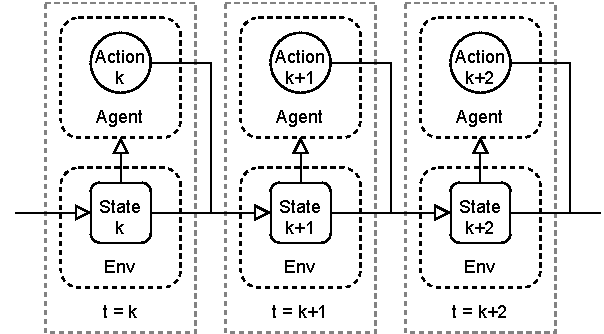
\includegraphics[width=0.75\textwidth]{figures/MDP.pdf}
    \caption{\acrfull{mdp}}
    \label{fig:mdp}
\end{figure}

\noindent
Assisting a human driver in the lane-keeping task is essentially a sequential decision-making task. However, the agent assisting the human driver does not know about the driver's internal psychological state. This state includes everything that influences the driver's behavior, such as the driver's goals, intentions, emotions, and perceptions, but is not visible from the outside world. We focus on the driver's attention to the driving task when referring to her hidden psychological state hereafter. A distracted driver may steer poorly and needs assistance. But how can the agent tell whether the driver is distracted? Reading the driver's mind is not feasible, and even if it were, it would be too invasive for this task. Instead, the agent needs to estimate the driver's internal state to act adequately. A \Glsentryfull{pomdp} is a generalization of an MDP that allows planning under uncertainty. Even without observing the complete state of the agent's environment, a POMDP enables the agent to estimate the environment's true state using the partial information it observes. In the next section, we will give a formal definition of a POMDP.

\section{Partially observable Markov decision process (POMDP)}
\label{sec:pomdp}

A POMDP is a generalization of an MDP for planning under uncertainty. The environment's true state is unknown to the agent. It has to rely on observations with partial information about the environment's true state to choose its actions. We follow the description in \cite{pomdp-definition} and define a POMDP as a tuple $(S, A, T, R, O, Z)$, where:
\begin{itemize}
    \item $S$ is the set of all possible states $s \in S$ of the environment. A state describes the environment at a time point. It must not be an all-encompassing description but must include all relevant information to make decisions. The state is hidden from the agent. This is the main difference to an MDP.
    \item $A$ is the set of all possible actions $a \in A$ the agent can perform in the environment.
    \item $T : S \times A \times S \rightarrow [0,1]$ defines the conditional state transition probabilities. $T(s,a,s') = Pr(s' | s, a)$ constitutes the probability of transitioning to state $s'$ after performing action $a$ in state $s$.
    \item $R : S \times A \rightarrow \R$ is the reward function providing the agent with a reward of $R(s,a)$ after performing action $a$ in state $s$.
    \item $O$ is the set of all possible observations $o \in O$. Observations are the agent's source of information about the environment, enabling the agent to estimate the environment's state.
    \item $Z : S \times A \times O \rightarrow [0,1]$ defines the conditional observation probabilities. $Z(s', a, o) = Pr(o | s', a)$ represents the probability of receiving observation $o$ at state $s'$ after performing action $a$ in the previous state. 
\end{itemize}

\noindent
At any time, the environment is in a certain state $s$. Unlike in the case of an MDP, the agent cannot directly observe the environment's state. Instead, the agent receives an observation $o$ that provides partial information about the current state. The agent uses the observations it perceives over time to estimate the true state of the environment to choose adequate actions. At any time step $t$, it takes into account the complete history $h_t$ of actions and observations until $t$:

\begin{equation}
    h_t = \{a_0,o_1,...,o_{t-1},a_{t-1},o_t\}
\end{equation}

Keeping a collection of all past observations and actions is very memory expensive. A less memory-demanding alternative is to only keep a probability distribution over the states at every step, called a belief $b$. The probability of being in state $s$ given history $h$ is denoted as $b(s,h)$. 

\begin{equation}
    b_t(s,h) = Pr(s_t = s|h_t = h)
\end{equation}

The belief is a sufficient statistic for the agent to form a decision about its next action \parencite{pomdp-belief}. Thus, only the belief needs to be kept and can be recursively updated whenever the agent performs an action and receives a new observation. The agent starts with an initial belief $b_0$ about the initial state of the environment. At every subsequent time step, the new belief $b'$ can be recursively calculated based on the previous belief $b$, the last action $a$, and the current observation $o$. The previous belief can then be discarded as the history it represents is no longer up-to-date. For an exact update of the belief, one can apply the Bayes theorem:

\begin{equation}
    \label{eq:bayes_update}
    \begin{split}
        b'(s') & = Pr(s' | o, a , b) \\
               & = \frac{Pr(o | s', a, b)Pr(s' | a,b)}{Pr(o| a, b)} \\
               & = \frac{Pr(o | s', a)\sum_{s \in S}Pr(s' | a, b, s)Pr(s| a, b)}{Pr(o| a, b)} \\
               & = \frac{Z(s', a, o)\sum_{s \in S}T(s, a, b)b(s)}{Pr(o | a, b)}
    \end{split}
\end{equation}

\noindent
The agent chooses its actions based on its belief according to its policy $\pi: b \rightarrow a$. The agent's policy defines the action to choose at any given belief state. It describes the strategy for every possible situation the agent can encounter. Solving a \gls{pomdp} consists in finding an optimal policy $\pi^*$ that maximizes the cumulative reward obtained over some time horizon $N$ starting from initial belief $b_0$ using a discount factor $0 \leq \lambda \leq 1$:

\begin{equation}
    \pi^* = argmax_{\pi}~E\left[ \sum_{t=0}^{N} \sum_{s \in S}b_t(s) \sum_{a \in A} \lambda^t R(s,a) \pi(b_t,a) | b_0\right]
\end{equation}

\noindent
The return gained by following a policy $\pi$ from a certain belief $b$ can be obtained with the value function $V^\pi(b)$:

\begin{equation}
    V^\pi(b) = \sum_{a \in A} \pi(b,a) \left[ \sum_{s \in S} b(s) R(s,a) + \lambda \sum_{o \in O} Pr(o | b, a) V^\pi(b')\right]
\end{equation}

\noindent
The optimal policy $\pi^*$ maximizes $V^\pi(b_0)$. For any POMDP, there exists at least one optimal policy.

\section{Key challenges}
\label{sec:challenges}

\subsection{Curse of dimensionality and curse of history}
\label{sec:curses}

Computing an optimal policy for a POMDP is challenging for two distinct but interdependent reasons \parencite{pomdp_curses}. On the one hand, there is the so-called curse of history: Finding an optimal policy means searching through the space of all possible action-observation histories. The number of distinct histories grows exponentially with the size of the time horizon. Therefore, planning further into the future increases the computation complexity exponentially. Finding an optimal policy can be relatively easy for short histories. However, it becomes computationally infeasible for larger time horizons. On the other hand, there is the curse of dimensionality: The belief space is $|S|$-dimensional. Therefore, the size of the belief space, representing the number of states in a POMDP, grows exponentially with $|S|$. For a POMDP with a large state space or time horizon, finding an optimal policy is computationally infeasible \parencite{pomdp_complex}. For this reason, approximate algorithms are often applied.  We summarize those approximate algorithms in section \ref{sec:solvers}.

\subsection{Unknown transition and observation probabilities}
\label{sec:gen_model_intro}
For many problems, it is difficult or impossible to know the probability distributions $T$ or $Z$ explicitly. This is also the case for the shared control lane-keeping scenario assessed in this thesis. Neither the transition probabilities nor the observation probabilities are known a priori. The belief update method using Bayes' theorem presented in Equation \ref{eq:bayes_update} is not computable without knowing the probability distributions explicitly. However, exact updates are too complex for problems with large state spaces in general \parencite{pomcp}. 

Some solution approaches circumvent the problem of unknown transition and observation probability distributions by using a generative model to sample state and observation transitions. This generative model can, given the current state and action, stochastically generate a successor state, reward, and observation. Thereby, it implicitly defines the transition and observation probabilities, even if they are not explicitly known. In this thesis, we follow this idea and employ a generative model to solve this challenge in our practical task. The generative model is described in detail in section \ref{sec:gen_model}.

\section{Algorithms to approximately solve large POMDPs}

\subsection{Offline and online POMDP solving}
\label{sec:on-off}

\begin{figure}[htbp]
    \centering
    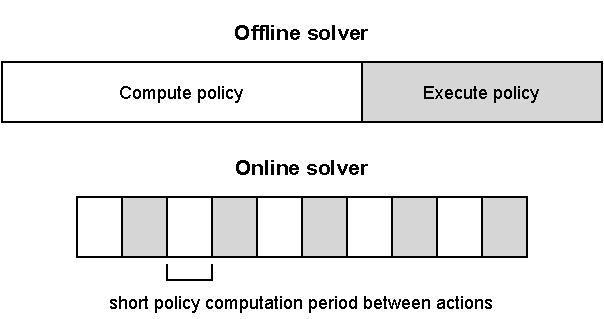
\includegraphics[width=0.6\textwidth]{figures/online-offline.pdf}
    \caption{Comparison of offline and online solving procedure}
    \label{fig:online-offline}
\end{figure}

\noindent
There are two general approaches to solve POMDP: offline and online (see figure \ref{fig:online-offline}). Offline solvers compute the optimal policy prior to execution for all possible future scenarios. Their advantage is that once the policy is determined, policy execution is fast as there is only a very minimal, negligible time overhead. However, offline planning is hard to scale to complex problems as the number of possible future scenarios grows exponentially with the size of the time horizon (curse of history). Furthermore, while the performance for small to medium-sized POMDPs can be good, computing the policy may take a very long time. Furthermore, even small changes in the dynamics of the environment require a full recomputation \parencite{online_pomdp}. Online solvers interleave planning and plan execution. At every time step, only the current belief is considered for the computation of the next optimal action by searching ahead until a certain depth is reached. On the one hand, the scalability is greatly increased. On the other hand, sufficiently more online computation than for offline planning is required. The amount of available online planning time at each time step limits the performance. 

\subsection{Overview of aproximate POMDP solvers}
\label{sec:solvers}

As discussed in section \ref{sec:curses}, finding an exact optimal policy is only feasible for small discrete POMDPs. Larger POMDPs are usually solved approximately. A wide range of offline and online approximate solvers is available. An extensive survey of possible approaches is out of scope for this thesis. A good overview over different methods is given in the book "Algorithms for Decision Making" \parencite{decision_making_book}. We focus on introducing a selection of especially noteworthy approaches at solving POMDP in this section.

For discrete POMDP, the most effective offline approximate solvers apply a form of \gls{pbvi}, where only a representative subset of the belief space is considered to approximate the value function \parencite{pomdp-point-based-value}. State of the art methods include Perseus \parencite{pomdp_perseus}, and \gls{hsvi} \parencite{solver_hsvi}. Perseus chooses belief states by randomly sampling trajectories from an initial belief \parencite{pomdp_perseus}. It is sufficiently more compute efficient than PBVI but can suffer from a slow convergence behavior \parencite{pbvi-survey}. HSVI improves on Perseus potential slow convergence in large domains by constructing a belief search tree, maintaining the order of visited beliefs to be backtrack value updates bottom-up \parencite{solver_hsvi}. Even the most advanced offline solvers reach their limit when dealing with POMDPs with large state spaces. As the state space for the shared control lane-keeping task is large, offline solvers are not considered further in this thesis. 

When it comes to online solvers, the paradigm of searching for a good policy locally for the current belief state makes them sufficiently more efficient. The general approach is to construct a search tree with the current belief as root, evaluating all possible further actions and observations. This tree can be used to efficiently generate a good approximately optimal action to perform at the current belief. The methods mainly differ in how the tree is constructed. After an action has been performed in the real environment, the agent receives a reward and observation. On this basis, it updates its belief, and the process repeats from the new belief. 

Constructing the search tree using Monte Carlo sampling has recently led to promising results for online solving of large POMDPs \parencite{pomcp}. Including all possibilities in the search tree is not feasible for deep time horizons because of the curse of history and the curse of dimensionality (see section \ref{sec:curses}). \gls{mcts} methods address this issue by using a generative model to sample state transitions and observations (see section \ref{sec:gen_model_intro}). By doing so, only a subset of histories is considered. The curse of dimensionality can be overcome in a similar fashion. Instead of evaluating all belief states, the start states for the search tree are sampled from the belief space. The number of belief states to consider can thereby be drastically reduced. 

\subsection{Online POMDP solving using Monte Carlo tree search}

The approach of using Monte Carlo sampling for both the choice of evaluated histories and estimating the belief was first applied in the \Glsentryfull{pomcp} algorithm by \cite{pomcp}. The exploration is controlled using the \gls{ucb1} \parencite{ucb1} algorithm for action selection. The belief search tree is constructed by sampling possible action-observation trajectories. The key idea is to approximate the belief space using the same set of states sampled for the search tree construction. POMCP's belief representation eliminates the need for expensive belief update calculations. POMCP has successfully been applied to solve large POMDPs. Thus, the POMCP algorithm was selected as the solver for our problem. In section \ref{sec:pomcp}, we explain how we employed POMCP to solve the shared control lane-keeping task. 

The \gls{despot} algorithm by \cite{despot} is a similar approach that can be seen as an evolution of POMCP. DESPOT is efficient as only a fixed number of sampled scenarios are considered. A scenario is a determinized trajectory in the belief tree that is defined in advance. At every depth of the belief tree, all actions but only a subset of resulting observations are considered. Thereby, the observation space is simplified. DESPOT's main advantage over POMCP is the ability to overcome POMCP's relatively poor worst-case behavior \parencite{pomcp-worst-case} caused by the UCB1 algorithm's tendency to overfit. DESPOT circumvents this by using regularization in the value function. First, a suboptimal policy is searched using heuristic search \parencite{solver_hsvi} and then it is incrementally improved upon. Branch-and-bound pruning is performed by pruning action nodes from the tree if their expected value is lower than the lower bound of another action. There are further extensions of DESPOT: HyPDESPOT is a parallelized version of DESPOT with significant performance enhancements \parencite{hyp-despot}. DESPOT-$\alpha$ further improves DESPOT's capability to handle very large observation and state spaces \parencite{despot-a}. And DESPOT-IS applies importance sampling to account for very rare events that are hard to sample \parencite{despot-is}. Unfortunately, DESPOT and its derivatives require the observation probability $Z$ to be explicitly known. This is not feasible for the shared control lane-keeping task considered in this thesis.

\subsection{Solving continuous POMDP}

The scenario of lane-keeping with a human in the loop that we examine is naturally continuous; steering actions, car state, and sensory information about the car's position are all composed of continuous values (see section \ref{sec:lane_keeping_loop}). Hence, a solver that can handle continuous POMDP is required.

The aforementioned algorithms POMCP and DESPOT can natively handle continuous state spaces \parencite{pomcp_continuous}. It is unlikely that two identical continuous states are inserted into the collection of states representing the agent's belief. Therefore, the individual relative frequency of a state in the belief, representing its probability in the discrete case, is rendered meaningless. Nevertheless, if the agent samples multiple similar situations, the corresponding states are also similar. For the continuous case, the assumed probability of being in a certain state is given by the number of belief states close to it.

However, POMCP and DESPOT cannot be applied directly with PODMPs that have continuous action and observation spaces. Discretization is required \parencite{pomcp_continuous}. Action and observation discretization is performed in this thesis to be able to use POMCP. The details are discussed in section \ref{sec:discretization}.

Various solvers have been developed that are suitable to solve POMDP with continuous action and observation spaces without relying on discretization. To the best of our knowledge, they all require the observation probabilities $Z$ to be known explicitly and are therefore not applicable to the problem addressed in this thesis. Yet, such approaches may be advantageous in future work if the problem of unknown observation probabilities can be circumvented. Two notable solvers are POMCPOW \parencite{online_pomdp_cont}, and LABECOP \parencite{online-cont-pomdp-2}. POMCPOW is an extension of POMCP using progressive widening. It uses weighted belief updates and limits the number of observations considered during planning. LABECOP is based on MCTS as well but avoids limiting the number of considered observations.
    \chapter{Methodology}
\label{sec:problem}


% TODO: Page 38 of Improving Sequential Decision Making in Human-In-The-Loop Systems

% \begin{enumerate}
%     \item How to get transition and observation probabilities? Am I correct that these need to be given by Florian's model? How would this ever be known in the case of learning with real human drivers?
%     \item Is the Markov assumption satisfied even though the driver's attentiveness does not depend on the previous state and action?
%     \item What is known a priori?
%     \begin{itemize}
%         \item human's current action (assumption: no, for performance reasons)
%         \item reward function
%     \end{itemize}
% \end{enumerate}

\section{Lane keeping with a human in the loop as a POMDP}

% TODO: Add overview picture

% TODO: Add: The agent can only recognize a state change of the driver after the driver has performed the first action in this state. This is because there are no observable clues about the duration of the driver's attentiveness and distraction.

\subsection{Driving simulator TORCS}

\subsubsection{State}

% TODO: Define terminal state

The tracks will be round courses. Thus, there is no terminal state if everything goes well. If the car reaches an off-track position, however, the car is reset to be in the initial starting position again.\\

\begin{tabularx}{\textwidth}{@{}p{0.18\textwidth}>{\centering}p{0.22\textwidth}X@{}}
\toprule
\textbf{Name}           & \textbf{Measurement}          & \textbf{Description}                                           \\ \midrule

Gear \newline \textbf{(constant)} & \{$-1$, $0$, $1$,  \dots, $6$\} & Distance of the car from the start line along the track line. \textbf{Neither the human driver nor the agent can directly influence this with their actions.} \\ \midrule

RPM \newline \textbf{(constant)} & [0, $+\inf$) & Number of engine rotations per minute. \textbf{Neither the human driver nor the agent can directly influence this with their actions.} \\ \midrule

Speed \newline \textbf{(constant)}  & ($-\inf$, $+\inf$) (km/h) & Speed along the longitudinal axis of the car. \textbf{Neither the human driver nor the agent can directly influence this with their actions.} \\ \midrule

% Lift \newline \textbf{(constant)} & ($-\inf$, $+\inf$) (km/h) & Speed along the vertical axis of the car. Will be zero as we use completely flat terrain. \textbf{Neither the human driver nor the agent can directly influence this with their actions.} \\ \midrule

Side force & ($-\inf$, $+\inf$) (km/h) & Speed along the transverse axis of the car. This is directly influenced by the steering actions of both human driver and agent. \\ \midrule

Distance from start & [0, $+\inf$) (m) & Distance of the car from the start line along the track line. \\ \midrule

Angle          & [$-\pi$, $+\pi$] (rad) & Angle between car direction and track axis direction.  \\ \midrule

Lane position & ($-\inf$, $+\inf$)     & Horizontal distance between the car and the track axis. $0$ when the car is on the axis, $+1$ if the car is on the left edge of the track, and $-1$ if the car is on the right edge of the track. Greater numbers than $+1$ or smaller numbers than $-1$ indicate that the car is off-track. \\ \midrule

Driver attention & True / False & Whether the human driver is attentive or distracted.  \\ \bottomrule

\end{tabularx}

\subsubsection{Actions}

\begin{tabularx}{\textwidth}{@{}p{0.18\textwidth}>{\centering}p{0.22\textwidth}X@{}}
\toprule
\textbf{Name}           & \textbf{Measurement}          & \textbf{Description}\\ \midrule

\multicolumn{3}{@{}>{\centering}p{\linewidth}@{}}{\textit{In our simplified scenario, both the human driver and the agent can not accelerate, brake or switch gears.}} \\ \midrule

Steering         & [$-2$, $+2$] & The input to the car is generated by combining the agent's action with the human's steering action (see equation~\ref{eq:steering}). For the car,  $-1$ means full right (159 degrees) and $+1$ means full left (21 degrees). A value greater than +1 or lower than -1 can effectively reverse an opposite action of the human driver. \\ \bottomrule
\end{tabularx}\\\\

\noindent The human driver and the agent share control of the steering wheel. The speed of the car is fixed and cannot be altered; neither by human driver nor agent. The steering input of the driver $\mathcal{A}_{steer}^{driver}$ and agent $\mathcal{A}_{steer}^{agent}$ are combined to ${A}_{steer} \in [-1, +1]$ using equation~\ref{eq:steering}.

The agent needs to be able to fully counteract a distracted driver's actions. In the extreme case, while the car is in a curve, a distracted driver could steer into the opposite direction of the trajectory of the lane center. Thus, the car would not only diverge from the lane center but would even get off the road completely. The agent thus needs to reverse the driver's action in order to keep the car centered in the lane and follow the road curve. Therefore, we define the range for the agent's steering action as follows: $\mathcal{A}_{steer}^{agent} \in [-2, +2]$.

\begin{equation}
    \mathcal{A}_{\textrm{steer}} = \min(\, -1, \, \max(\, 1, \, (\mathcal{A}_{\textrm{steer}}^{\textrm{driver}} + \mathcal{A}_{\textrm{steer}}^{\textrm{agent}})\,)\,)
    \label{eq:steering}
\end{equation}

\subsubsection{Observations}
\label{sec:observations}

\begin{figure}[ht]
    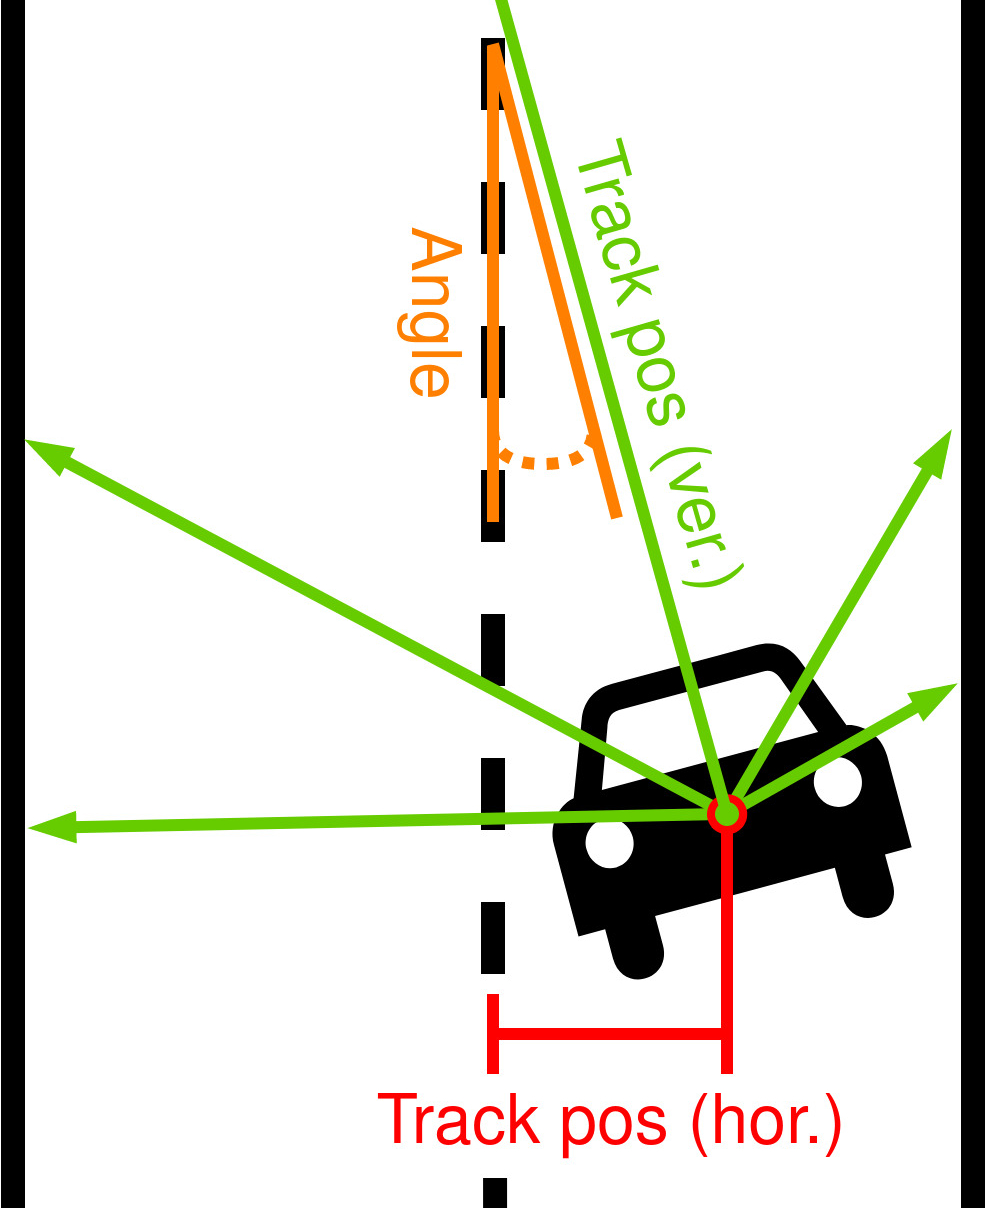
\includegraphics[width=0.3\linewidth]{figures/Observations.jpg}
    \centering
    \caption{Main environment observations}
    \label{fig:observations}
\end{figure}


\begin{tabularx}{\textwidth}{@{}p{0.18\textwidth}>{\centering}p{0.22\textwidth}X@{}}
\toprule
\textbf{Name}           & \textbf{Measurement}          & \textbf{Description}   \\ \midrule

\multicolumn{3}{@{}>{\centering}p{\linewidth}@{}}{\textit{Constant state parameters are not observed as they do not influence learning.} \textbf{The observations are not noisy.}} \\ \midrule

Angle          & [$-\pi$, $+\pi$] (rad) & Angle between car direction and track axis direction  \\ \midrule

Side force & ($-\inf$, $+\inf$) (km/h) & Speed along the transverse axis of the car. This is directly influenced by the steering actions of both human driver and agent. \\ \midrule

Track position (horizontal) & ($-\inf$, $+\inf$)     & Horizontal distance between the car and the track axis. $0$ when the car is on the axis, $+1$ if the car is on the left edge of the track, and $-1$ if the car is on the right edge of the track. Greater numbers than $+1$ or smaller numbers than $-1$ indicate that the car is off-track.  \\ \midrule

Track position (vertical)  & [$0$,$200$] (m) & Vector of 5 range finder sensors (of 19 available in TORCS). The range finders serve as lookahead by returning the distance between the car and the track edge in a given forward angle between $-90$ and $+90$ degrees with respect to the car axis. \\ \midrule 

Driver steering (last time step) & [$-1$, $+1$]  & The agent perceives the last input of the human. This is not the action of the human in the next but in the last time step. The agent does not know which action the human is going to choose simultaneous to its own action. $-1$ means full right (159 degrees) and $+1$ means full left (21 degrees).  \\ \bottomrule
\end{tabularx}

\subsection{Driver model}
\label{sec:driver_model}

The driver model is simplistic. If the driver is attentive, its actions are optimal. The driver model returns the action that steers the car as close to the center of the lane as possible. In this case, the agent should not interfere. However, if a distracted driver is modeled, the driver just repeats the last action it performed while being attentive. This can have the effect of the driver's action to overshoot with the car diverging from the center of the lane. Following, the agent has to identify distracted driving and counteract.

When the driver model is initialized, it is randomly set to be attentive or distracted. The driver stays in this state for a randomly chosen discrete time period between ten and 60 seconds for an attentive state and between two and six seconds for a distracted state. After the chosen time period, the state of attentiveness switches; a previously attentive driver becomes distracted, and a previously distracted driver becomes attentive. The process repeats until the experiment is over.

\subsubsection{Simple driver model}


\subsubsection{Steering over-correction}


\subsubsection{Steering over-correction and noise}

\subsection{Reward}

The overall goal for the agent is to only assist the driver in keeping the car centered in its lane. Therefore, this is the main source of reward for the agent. The more centered the car is at a certain time step, the more reward $r$ is received. However, the agent is supposed to leave the human driver with as much autonomy as possible. Thus, any intervention by the agent is penalized. Minor smooth interventions are generally preferred over large abrupt steering actions. Accordingly, the penalty is (exponentially) dependent on the intensity of the agent's action. The general assumption is that an attentive driver performs better in keeping the car centered than an inattentive driver. The agent has to predict whether a driver is attentive or not in order to choose its actions correctly. An incorrect prediction of the driver's actions will lead to overshooting and thus be negatively reflected in the reward for keeping the car centered. Lastly, the car is never supposed to leave the lane. Consequently, leaving the lane is highly penalized.


%For this reason, the penalty intensity is linked to the current distance of the car to the lane center; the higher the distance, the lower the agent's intervention penalty. On the other hand, 

% TODO: Add smoothing?

% \begin{equation}
%     \mathcal{R} = \mathcal{R}_{\textrm{center}} - \mathcal{P}_{\textrm{act position}} - \mathcal{P}_{\textrm{act intensity}} - \mathcal{P}_{\textrm{off-lane}}
% \end{equation}
\begin{equation*}
    \mathcal{R} = \mathcal{R}_{\textrm{center}} - \mathcal{P}_{\textrm{act intensity}} - \mathcal{P}_{\textrm{off-lane}}
\end{equation*}
\begin{equation*}
    \mathcal{R}_{\textrm{center}} = 
    \begin{cases}
        r - r * |Pos_{hor}| & \text{if} \quad |Pos_{hor}| \leq 1 \\
        0 & \text{if} \quad \text{off-lane}
    \end{cases}
\end{equation*}
% \begin{equation}
%     \mathcal{P}_{\textrm{act position}} = 
%     \begin{cases}
%         p_{\textrm{pos}} - p_{\textrm{pos}} * |Pos_{hor}| & \text{if} \quad |Pos_{hor}| \leq 1 \text{ and } \mathcal{A}_{\textrm{steer}}^{\textrm{agent}} \neq 0 \\
%         0 & \text{if} \quad \text{off-lane or no steering action}
%     \end{cases}
% \end{equation}
\begin{equation*}
    \mathcal{P}_{\textrm{act intensity}} = |\mathcal{A}_{\textrm{steer}}| ^ {p_{\textrm{int}}}
\end{equation*}
\begin{equation*}
    \mathcal{P}_{\textrm{off-lane}} = 
    \begin{cases}
        p_{\textrm{off}} & \text{if} \quad |Pos_{hor}| > 1 \\
        0 & \text{if} \quad |Pos_{hor}| \leq 1
    \end{cases}
\end{equation*}

\section{Solution approach using the POMCP algorithm}
\subsection{Discretization}
\label{sec:discretization}

\subsection{General POMCP definition}
\label{sec:pomcp}

% explain: 
% - Planning versus learning
% - How POMCP breaks the curse of dimensionality with Monte-Carlo sampling
% - Belief and blief update

% Particle filter belief update:
% See (POMDP, Thesis) Tactical Decision-Making forHighway Driving

% TODO: Replace planning time with number of searches
% TODO: Add select random
% TODO: Fix arrow for h = hao, s=s' (Use two diagonal arrows)
% TODO: Add caption
% TODO: Mark rollout and search phase as in the original paper
\begin{figure}[htbp]
    \centerfloat
    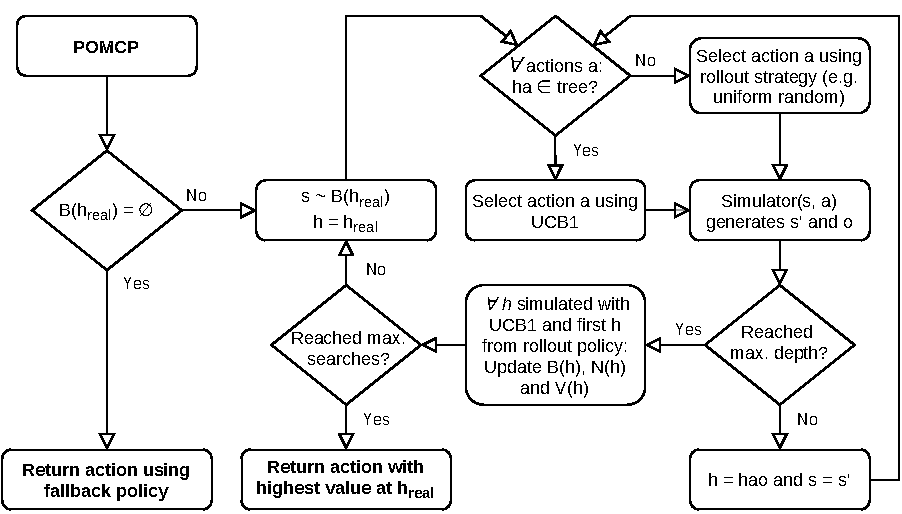
\includegraphics[width=1.2\textwidth]{figures/POMCP.pdf}
\end{figure}

\Gls{pomcp} constructs a search tree with nodes representing histories $h$ of actions and observations. At each node, $N(h)$ stores the number of times the represented history $h$ has been encountered, $V(h)$ is the node's value that is approximated by the average return of simulations starting at history $h$, and $B(h)$ represents the node's belief over the real environment's state. $B(h)$ is a collection of potential states where the likelihood of each state is given by the relative number of times it is included in the collection.

If the belief at the node representing $h_{real}$ is empty, an initial state distribution $I$ is used to sample a start state $s$ for the search. Otherwise, $B(h_{real})$ is utilized. The search tree is then searched in two stages. First, in the case that the search tree already contains child nodes for all actions at the current history, UCB1 is used for the action selection. Exploration is achieved by increasing the value of rarely-tried actions by an exploration bonus. Second, when the tree is missing a node for a potential action at the current history, a rollout policy is used to select actions. In the most simple case, this means choosing uniformly random over the action space. In either case, the selected action is executed on the start state $s$, leading to a successive state $s'$, observation $o$, and reward $r$. The process is repeated with resulting successive states until a maximum depth of the tree is reached. Afterwards, the beliefs, counts, and values are updated at all nodes for the histories resulting from the UCB1 action selection, and the node for the first history resulting from the rollout policy. The belief is updated by adding the successive states $s'$ from the simulator to the collections $B(ho)$ in the nodes. If the maximum planning time has not yet been reached, another start state is sampled and the whole process repeats. When the time runs out, the action $a_{best}$ with the highest value at the current history $h_{real}$ is returned. After this action is executed in the real environment, with an observation $o_{last}$ the tree can be pruned. Only the nodes from history $h_{real}a_{best}o_{last}$ onward stay relevant as all other histories are rendered impossible.

% TODO: Add particles as a construct (Or change particles everywhere else to "state in the belief")
% See Algorithms for decision making book

% One common approach is to use a particle filter, which represents the belief state as a collection of states. 10 Each state in the approximate belief is called a particle.

\subsection{Particle deprivation and particle injection}
\label{sec:particle_deprivation}

Particle filter approaches, POMCP included, can fail due to a phenomenon called particle deprivation. Because of the random nature of the process, the belief can sometimes converge towards a state that is far from the environment's true state. Particles that differ from the converged state have a low probability to be selected while sampling (low relative count). Hence, with each iteration, they become scarcer until they are completely erased from the belief. At this point, the agent is sure to be in an erroreous state and cannot recover anymore. Particle injection (also called particle reinvigoration) is a method to counteract this problem by introducing a number of random particles to the belief at each iteration \parencite{decision_making_book}. While this reduces the accuracy of the belief, it prevents its complete convergence towards a wrong state. 

Particle injection is used to increase the variance of the belief about the driver model state. Only observable information is used. Concretely, particle injection is implemented by adding driver model states with a random number of remaining actions and the same action as the one that was last observed. The number of remaining actions can be lower than the minimum defined in Section~\ref{sec:driver_model} because this limit is only intended for initial sampling and the true remaining number of driver actions in a particular state might be lower after having performed actions already. Like in the original POMCP paper, the amount of transformed particles that are added before each planning step is $1/16$ of the number of searches. The particles can be added during policy execution, and therefore, do not influence planning time.

% Use term posterior probability distribution? We can only add particles after making an observation so that we can verify that the potential particles to add match this belief.


\subsection{Action selection and preferred actions}
\label{sec:action_selection}

% TODO: Just say the agent does not act anymore when losing track with the belief instead of using uniformly random action selection? Makes more sense.

% This is strongly related to the particle deprivation problem described in Section~\ref{sec:particle_deprivation}. When the driver is in a distracted or attentive state, any number of remaining actions in this state below the maximum number (see Section~\ref{sec:driver_model}) could be valid and can therefore be part of the driver model states in the belief. In successive iterations, particles that represent drivers switching their state earlier than the true driver, and therefore change their steering behavior, are ruled out and removed from the belief. Thereby, after some iterations, driver model states that have the same or more remaining actions than the true state dominate the belief.

% preferred actions = domain knowledge


    \chapter{Experimental setup}
\label{sec:setup}

% TODO: Define terminal state

% TODO: Refine
The task for the agent in the experiment is to keep the car centered in a highway lane. Thus, the track used for the agent's evaluation needs to represent such a scenario. Most tracks readily available in the racing car simulator TORCS are race tracks. These are much wider than common roads and the width often differs in different segments. To ensure a realistic scenario, a one-lane track with a continuous width of 3.5m, which is common for European roads, is used. The track covers a wide array of scenarios. It includes long straight segments, both left and right curves, and multiple curves of alternating directions in a row. By ensuring that all common highway scenarios are covered by the track, a single track is sufficient.

The car used for the experiment does not have a big impact on driving performance, as long as it is consistent during all experiments. To ensure that an action's effect at a particular position are consistent, the speed of the car is constant.

The driver is pulled for an action every 0.1 seconds. The simulation tick rate is 0.002 seconds. When the driver is not pulled, its last action is repeated. It follows, that every action is repeated during 50 simulation ticks. The simulation is not in real time. Therefore, the simulation waits for the agent's planning. If the agent is pulled for an action, the environment does not change until the agent's next action is decided and performed.

\section{Evaluated scenarios}
\subsection{Driver model}
\subsection{Action space and action selection}
\section{Design decisions}
% TODO Leave out? Or add something useful here

\section{Hyperparameter optimization}

% TODO: Add parameter and hyperparameter table

% TODO: Refine
There are a number of hyperparameters. Most importantly, there is the planning time. This is the time the agent is allowed to search in and expand its search tree in order to find the most likely current state and best course of action. More planning time can result in a wider and/or deeper tree. The search horizon is limited by a discount threshold. If this threshold is reached, the search is stopped and no more actions will be performed for the current trajectory and, if there is enough planning time left, a new state is sampled from the current belief and a new planning trajectory is expanded. Moreover, there is an exploration constant. This value, determined before the start of the experiment, assigns actions that have not been tried before more expected reward and thus favors exploration.
\subsubsection{Number of searches}
\subsubsection{Exploration constant}
\subsubsection{Discount horizon}

\section{Performance metrics}
Due to the randomness involved in the driver model, each experiment run will lead to a different scenario. Therefore, to get credible results, the experiment has to be repeated many times. The average discounted return over all experiment runs serves as performance metric. This result is compared with the average reward of an agent that always performs the optimal reaction to the action of the driver model. The closer the POMCP agent's reward is to the optimal agent's reward, the better was the planning.


    \chapter{Results}
\label{ch:results}

\section{Lower and upper performance bound}

The benchmarks for the performance of the agent are the performance of the driver without assistance system as lower bound, and the performance of an agent that always reacts optimally to the driver's actions as upper bound. For both baselines, 50 runs with up to 1000 actions each, if no terminal state is reached earlier, are performed for each of the three driver models. 

In the case of the independent driver, no run was completed successfully. At some point in any run the driver becomes distracted and fails to adjust to a change of the course of the road, leading to lane departure. Table \ref{tab:driver_performance} shows that the more complex the driver model is, the worse is its performance. The simple driver model and the driver model with steering overcorrection lead to a few runs with a relatively high number of successful actions before a lane departure occurs. The reason for this is that the driver only repeats it's last attentive action after becoming distracted. In some cases this means that the distracted driver just continues to steer straight which is less likely to lead to lane departure on the highway track than consecutively steering left or right.

The agent that reacts optimally to the driver's actions has full knowledge about the environment, as well as the driver's next action and is equipped with a continuous optimal steering policy. Therefore, it can easily choose its action by checking which combined action is the closest to the optimal steering. Due to the discretization of the action space, a possible combination that equals the optimal steering is unlikely but the agent performs whatever action leads to the closest result. It finishes every run successfully and leads to average cumulative rewards of $999.3$ for all driver models.

\begin{table}[htbp]
\footnotesize
\centering
\begin{tabular}{@{}rccc@{}}
\toprule
                            & Mean reward & Min \texttt{\#}actions & Max \texttt{\#}actions \\ \midrule
Simple driver               & 54.39       & 17                     & 347                    \\
Over correction             & 51.26       & 17                     & 233                    \\
Over correction and noise   & 31.08       & 14                     & 74                     \\ \bottomrule
\end{tabular}
\caption{Independent driver performance}
\label{tab:driver_performance}
\end{table}

\section{Hyperparameter optimization}

Hyperparameter optimization is performed for agents with all three action configurations and the driver model with steering overcorrection but without noise. Grid search is used to search for the combination of search horizon and exploration constant that leads to the highest average cumulative reward after 20 runs with up to 1000 actions each and 1000 searches per planning step.

\begin{figure}[htbp]
    \centering
    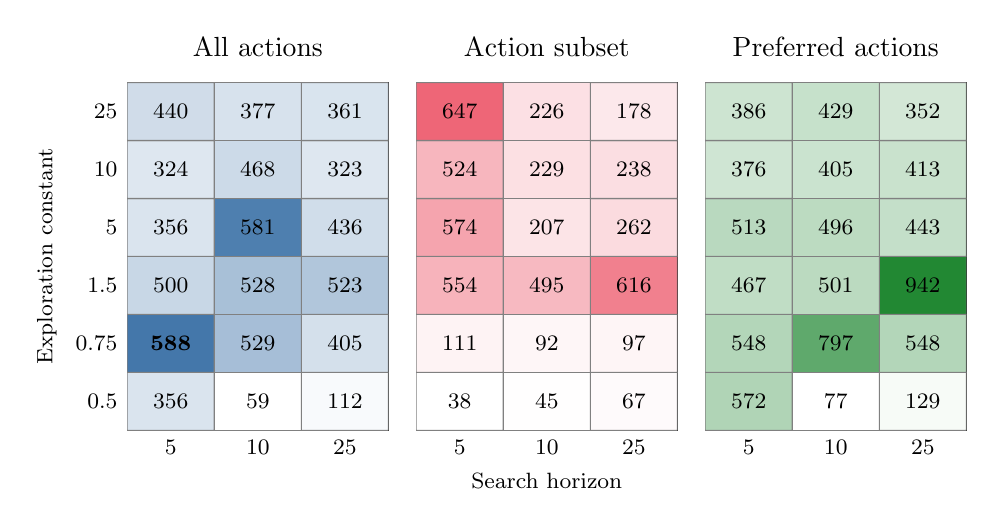
\begin{tikzpicture}
        \begin{groupplot} [
            group style={
                group name=grid group,
                group size=3 by 1,
                ylabels at=edge left,
                yticklabels at=edge left,
                horizontal sep=10pt
            },
            width=4.9cm,
            height=6cm,
            enlargelimits=false,
            ylabel=Exploration constant,
            yticklabels={0.5, 0.75, 1.5, 5, 10, 25},
            ytick={0,...,5},
            ytick style={draw=none},
            xticklabels={5, 10, 25},
            xtick={0,...,2},
            xtick style={draw=none},
            xlabel style={font=\footnotesize},
            ylabel style={font=\footnotesize},
            legend style={font=\footnotesize},
            xticklabel style={font=\footnotesize},
            yticklabel style={font=\footnotesize},
            nodes near coords={\ifdim \Cvalue pt = 587.674 pt {\textbf{\pgfmathprintnumber[assume math mode=true, precision=0]\Cvalue}} \else {\pgfmathprintnumber[assume math mode=true, precision=0]\Cvalue} \fi},
            visualization depends on={\thisrow{C} \as \Cvalue},
            nodes near coords style={anchor=center, font=\footnotesize}
        ]
        \nextgroupplot[title=All actions]
        \addplot[
                matrix plot*,
                mesh/cols=3,
                point meta=explicit,
                draw=gray,
                colormap={whitemyblue}{color(0)=(white), color(500)=(myblue!30), color(587)=(myblue)}
            ] table [meta=C] {
                x y C
                0 0 356.159
                1 0 59.1294
                2 0 112.128

                0 1 587.674
                1 1 529.063
                2 1 404.732

                0 2 499.689
                1 2 528.001
                2 2 522.667

                0 3 355.745
                1 3 581.4
                2 3 436.268

                0 4 323.708
                1 4 467.673
                2 4 323.037

                0 5 439.826
                1 5 377.36
                2 5 360.914
            };
        \nextgroupplot[title=Action subset, xlabel=Search horizon]
        \addplot[
                matrix plot*,
                mesh/cols=3,
                point meta=explicit,
                draw=gray,
                colormap={whitegreen}{color(0)=(white), color(400)=(myred!40), color(550)=(myred!50), color(646)=(myred)},
            ] table [meta=C] {
                x y C
                0 0 37.504
                1 0 45.359
                2 0 67.388

                0 1 110.563
                1 1 91.882
                2 1 96.874

                0 2 553.591
                1 2 494.649
                2 2 616.474

                0 3 573.726
                1 3 206.534
                2 3 261.538

                0 4 524.302
                1 4 228.895
                2 4 238.421

                0 5 646.833
                1 5 225.915
                2 5 177.826
            };
        \nextgroupplot[title=Preferred actions]
        \addplot[
                matrix plot*,
                mesh/cols=3,
                point meta=explicit,
                draw=gray,
                colormap={whitegreen}{color(0)=(white), color(600)=(mygreen!40), color(942)=(mygreen)}
            ] table [meta=C] {
                x y C
                0 0 572.054
                1 0 77.416
                2 0 128.668

                0 1 547.758
                1 1 796.5
                2 1 548.097

                0 2 466.936
                1 2 501.059
                2 2 942.054

                0 3 512.66
                1 3 496.409
                2 3 443.296

                0 4 375.698
                1 4 404.609
                2 4 413.298

                0 5 385.954
                1 5 429.494
                2 5 351.699
            };
        \end{groupplot}
    \end{tikzpicture}
    \caption{Average cumulative rewards for combinations of search horizon and exploration constant for all three action configurations (20 runs with up to 1000 actions each and 1000 searches per planning step; driver model with steering overcorrection but without noise).}
\end{figure}

For the agent with a full, unweighted action space, two combinations lead to a sufficiently higher average cumulative reward than the others: The combination of a search horizon of 5 actions with an exploration constant of 0.75 leads to a reward of 587.67, and the combination of planning 10 actions ahead with an exploration constant of 5 results in a reward of 581.40. The shallower the search horizon, the less planning time is needed at every planning step as fewer actions need to be simulated. Thus, at the same performance, a lower search horizon is preferable. The combination of a search horizon of 5 actions and an exploration constant of 0.75 is used for the further experiments.

In the case of the agent restricted to using a subset of the action space, the combination of a search horizon of 5 actions and an exploration constant of 25 yields the highest average cumulative reward of 646.83. Only the combination of looking ahead five actions with an exploration constant of 1.5 comes relatively close with a reward of 616.47. As a lower search horizon is preferable, the setup for the further evaluation for this agent is a search horizon of 5 actions with an exploration constant of 25. 

The best combination of search horizon and exploration constant for the agent with preferred actions is 25 actions and 1.5 respectively. This combination yields an average cumulative reward of 942.05 which is sufficiently higher than the return of any other combination. Consequently, this is the combination used for this agent in subsequent experiments.

\section{Convergence behavior}

% TODO: Show how many terminal states were reached

\subsection{Simple driver model}

% Add #actions while attentive

The simple driver model steers optimally when it is in an attentive state. In a distracted state, it simply repeats the last action it has performed while it was still attentive until it becomes attentive again. Therefore, the optimal policy for the agent is to only interfere when the driver is distracted. 

The challenge is threefold: First, the agent must accurately determine where the car is located on the track. The observations the agent receives are accurate, however, because of the discretization, multiple actual positions map to the same observation (See Section \ref{sec:observations}). Second, the agent needs to estimate whether the driver is attentive or not. Third, the agent must decide on an appropriate action choice, taking into account future consequences of the chosen action. In order to achieve this, at each planning step, the agent can search ahead by simulating experiences based on its belief of the environment's and the driver's states. Performing more searches means evaluating more possible scenarios. In turn, more evaluated scenarios enable the agent to form a better policy and therefore selecting the better next action. However, after some amount of searches, the gained information from additional searches decreases and performance is expected to converge \parencite{pomcp}. The number of searches is directly related to the planning time. Planning time is a limiting factor for the application of a planner. Thus, knowing after how many searches the performance converges, and therefore being able to choose the minimal number of searches to perform for a good result, is critical.

\begin{figure}[htbp]
    \centering
    \begin{tikzpicture}
    \begin{axis}[
        width=0.8\linewidth,
        height=6cm,
        mark size=1pt,
        xlabel={Number of searches},
        xtick={10, 100, 200, 300, 400, 500, 750, 1000, 1500, 2500, 5000, 7500, 10000},
        xticklabels={10, 100, 200, 300, 400, 500, 750, 1000, 1500, 2500, 5000, 7500, 10000},
        x tick label style={rotate=60, anchor=east},
        symbolic x coords= {10, 100, 200, 300, 400, 500, 750, 1000, 1500, 2500, 5000, 7500, 10000},
        xmajorgrids=false,
        xminorticks=false,
        ylabel={Average cumulative reward},
        ymajorgrids=true,
        ytick distance=200,
        legend pos=south east,
        xlabel style={font=\footnotesize},
        ylabel style={font=\footnotesize},
        legend style={font=\footnotesize},
        xticklabel style={font=\footnotesize},
        yticklabel style={font=\footnotesize},
        error bars/y dir=both,
        error bars/y explicit,
        % title={Average planning time},
        % title style={font=\footnotesize, yshift=15pt},
        % extra x ticks={10, 100, 200, 300, 400, 500, 750, 1000, 1500, 2500, 5000, 7500, 10000},
        % extra x tick style={
        %     grid=none,
        %     tick label style={
        %         rotate=0,
        %         anchor=east,
        %         yshift={20pt},
        %         xshift={10pt},
        %         yshift={(\ticknum==0)*4pt}
        %     },
        %     tick pos = right,
        %     ticklabel pos = right,
        % },
        % extra x tick labels={0.004, 0.05, 0.08, 0.12, 0.15, 0.19, 0.27, 0.36, 0.55, 0.92, 1.83, 2.93, 3.75}
    ]
    \addplot [solid, color=myblue, mark=square] table [x=Simulations, y=Average Reward, y error=Standard Error, col sep=comma]{data/Simulations/Simulations - 50 runs - 1000 actions - discount horizon 5 - exp const 0.75 mean.csv};
    \addplot [solid, color=purple, mark=square] table [x=Simulations, y=Average Reward, y error=Standard Error, col sep=comma]{data/Simulations/Reduced Actions - 50 runs - 1000 actions - discount horizon 5 mean.csv};
    \addplot [solid, color=mygreen, mark=square] table [x=Simulations, y=Average Reward, y error=Standard Error, col sep=comma]{data/Simulations/Preferred - 50 runs - 1000 actions - discount horizon 25 - exp const 1.5 - reduced mean.csv};
    \addlegendentry{All actions}
    \addlegendentry{Action subset}
    \addlegendentry{Preferred actions}
    \end{axis}
    \end{tikzpicture}
    \caption[Performance of POMCP with a simple driver model]{Performance comparison of POMCP when utilizing all actions, an action subset, or preferred actions with a simple driver model. Each point shows the mean cumulative reward from 50 runs with 1000 actions each, if no terminal state is reached earlier.}
\end{figure}

Using the full action space, utilizing only the subset of minor steering actions, and employing preferred actions lead to similar results for the experiment with the simple driver model. Already with just 200 searches during planning, the average cumulative reward is above 600 for all agents. However, as it can be seen in table \ref{tab:simple_terminal}, the number of runs that lead to a terminal state is high. In the runs that result in a terminal state, the agents are able to assist the drivers well at first but suffer from belief divergence after some time. Then, their belief deviates noticably from the environmen's and driver's true state. The agents are not able anymore to make accurate assumptions about the state of the environment and whether the driver is attentive or not. Thus, they are rendered unable to take the right actions to keep the car centered. 

The agent using the full range of actions already causes only four terminal states with 300 searches whereas the other two agents need more searches to perform well. The best result for all three agents is achieved with 1500 searches. No run results in a terminal state. The the agent with full action space receives an average cumulative rewards of 957.83, the agent with a reduced action space yields 981.99, and the agent using preferred actions gains 973.88. 

For more searches, the average rewards are comparable, with the exception of the trials with 5000 and 7500 simulations for the agent with a complete action space. Four and six runs which reach terminal states respectively. In all cases, the terminal states are reached early - executing less than 50 actions before. The causes are extreme actions by the agent that lead to the opposite of optimal steering behavior. These actions completely overrule the driver who is even concentrated in three of the ten occasions. The reason for this is likely the combination of a poor belief that strongly deviates from the true state, and exploration to counteract this by acquiring more information. % TODO: Check if this checks out


\begin{table}[htbp]
\footnotesize
\centering
\centerfloat
\begin{tabular}{@{}rccccccccccccc@{}}
\toprule
                    & 10 & 100 & 200 & 300 & 400 & 500 & 750 & 1000 & 1500 & 2500 & 5000 & 7500 & 10000 \\ \midrule
All       & 50 & 50  & 22  & 4   & 4   & 3   & 3   & 1    & 0    & 1    & 4    & 6    & 1     \\
Subset     & 50 & 48  & 27  & 26  & 11  & 18  & 6   & 5    & 0    & 2    & 0    & 2    & 2     \\
Preferred & 50 & 50  & 32  & 13  & 8   & 4   & 1   & 3    & 0    & 0    & 1    & 0    & 0     \\ \bottomrule
\end{tabular}
\caption{Number of terminal runs by the number of performed searches at each planning step in the experiment with a simple driver model for agents with all three action space types.}
\label{tab:simple_terminal}
\end{table}


\subsection{Steering over-correction}

\begin{figure}[htbp]
    \centering
    \begin{tikzpicture}
    \begin{axis}[
        width=0.8\linewidth,
        height=6cm,
        mark size=1pt,
        xlabel={Number of searches},
        xtick={10, 100, 200, 300, 400, 500, 750, 1000, 1500, 2500, 5000, 7500, 10000},
        xticklabels={10, 100, 200, 300, 400, 500, 750, 1000, 1500, 2500, 5000, 7500, 10000},
        x tick label style={rotate=60, anchor=east},
        symbolic x coords= {10, 100, 200, 300, 400, 500, 750, 1000, 1500, 2500, 5000, 7500, 10000},
        xmajorgrids=false,
        xminorticks=false,
        ylabel={Average cumulative reward},
        ymajorgrids=true,
        ytick distance=200,
        legend pos=south east,
        xlabel style={font=\footnotesize, yshift=5pt},
        ylabel style={font=\footnotesize},
        legend style={font=\footnotesize},
        xticklabel style={font=\footnotesize},
        yticklabel style={font=\footnotesize},
        error bars/y dir=both,
        error bars/y explicit,
        % title={Average planning time},
        % title style={font=\footnotesize, yshift=15pt},
        % extra x ticks={10, 100, 200, 300, 400, 500, 750, 1000, 1500, 2500, 5000, 7500, 10000},
        % extra x tick style={
        %     grid=none,
        %     tick label style={
        %         rotate=0,
        %         anchor=east,
        %         yshift={20pt},
        %         xshift={10pt},
        %         yshift={(\ticknum==0)*4pt}
        %     },
        %     tick pos = right,
        %     ticklabel pos = right,
        % },
        % extra x tick labels={0.004, 0.05, 0.08, 0.12, 0.15, 0.19, 0.27, 0.36, 0.55, 0.92, 1.83, 2.93, 3.75}
    ]
    \addplot [solid, color=myblue, mark=square] table [x=Simulations, y=Average Reward, y error=Standard Error, col sep=comma]{data/Simulations/Over Correct - 50 runs - 1000 actions - discount horizon 5 mean.csv};
    \addplot [solid, color=purple, mark=square] table [x=Simulations, y=Average Reward, y error=Standard Error, col sep=comma]{data/Simulations/Reduced Actions - Over Correct - 50 runs - 1000 actions - discount horizon 5 mean.csv};
    \addplot [solid, color=mygreen, mark=square] table [x=Simulations, y=Average Reward, y error=Standard Error, col sep=comma]{data/Simulations/Preferred - Over Correct - 50 runs - 1000 actions - discount horizon 25 - exp const 1.5 - reduced mean.csv};
    \addlegendentry{All actions}
    \addlegendentry{Action subset}
    \addlegendentry{Preferred actions}
    \end{axis}
    \end{tikzpicture}
    \caption[Performance of POMCP with a driver that overcorrects when regaining attentiveness]{Performance comparison of POMCP when utilizing all actions, an action subset, or preferred actions with a driver model that over-corrects when it regains attention. Each point shows the mean cumulative reward from 50 runs with 1000 actions each, if no terminal state is reached earlier.}
    \label{fig:searches_over}
\end{figure}

\begin{table}[htbp]
\footnotesize
\centering
\centerfloat
\begin{tabular}{@{}rccccccccccccc@{}}
\toprule
& 10 & 100 & 200 & 300 & 400 & 500 & 750 & 1000 & 1500 & 2500 & 5000 & 7500 & 10000 \\ \midrule
All       & 50 & 50  & 49  & 45  & 42  & 46  & 42  & 41   & 35   & 13   & 4    & 5    & 6     \\
Subset    & 50 & 50  & 49  & 49  & 48  & 49  & 42  & 39   & 23   & 17   & 3    & 1    & 1     \\
Preferred & 50 & 50  & 49  & 42  & 35  & 29  & 10  & 3    & 0    & 0    & 0    & 0    & 0     \\ \bottomrule
\end{tabular}
\caption{Number of terminal runs by the number of performed searches at each planning step in the experiment with a driver model with steering over correction for agents with all three action space types.}
\label{tab:simple_terminal}
\end{table}

\subsection{Steering over-correction and noise}

\begin{figure}[htbp]
    \centering
    \begin{tikzpicture}
    \begin{axis}[
        width=0.8\linewidth,
        height=6cm,
        mark size=1pt,
        xlabel={Number of searches},
        xtick={10, 100, 200, 300, 400, 500, 750, 1000, 1500, 2500, 5000, 7500, 10000},
        xticklabels={10, 100, 200, 300, 400, 500, 750, 1000, 1500, 2500, 5000, 7500, 10000},
        x tick label style={rotate=60, anchor=east},
        symbolic x coords= {10, 100, 200, 300, 400, 500, 750, 1000, 1500, 2500, 5000, 7500, 10000},
        xmajorgrids=false,
        xminorticks=false,
        ylabel={Average cumulative reward},
        ymajorgrids=true,
        ytick distance=200,
        legend pos=south east,
        xlabel style={font=\footnotesize},
        ylabel style={font=\footnotesize},
        legend style={font=\footnotesize},
        xticklabel style={font=\footnotesize},
        yticklabel style={font=\footnotesize},
        error bars/y dir=both,
        error bars/y explicit
    ]
    \addplot [solid, color=myblue, mark=square] table [x=Simulations, y=Average Reward, y error=Standard Error, col sep=comma]{data/Simulations/Over Correct + Noise - 50 runs - 1000 actions - discount horizon 5 mean.csv};
    \addplot [solid, color=purple, mark=square] table [x=Simulations, y=Average Reward, y error=Standard Error, col sep=comma]{data/Simulations/Reduced Actions - Over Correct + Noise - 50 runs - 1000 actions - discount horizon 5 mean.csv};
    \addplot [solid, color=mygreen, mark=square] table [x=Simulations, y=Average Reward, y error=Standard Error, col sep=comma]{data/Simulations/Preferred - Over Correct + Noise - 50 runs - 1000 actions - discount horizon 25 - exp const 1.5 - reduced mean.csv};
    \addlegendentry{All actions}
    \addlegendentry{Action subset}
    \addlegendentry{Preferred actions}
    \end{axis}
    \end{tikzpicture}
    \caption[Performance of POMCP with a driver that overcorrects and steering noise]{Performance comparison of POMCP when utilizing all actions, an action subset, or preferred actions with a driver model that over-corrects when it regains attention and performs noisy actions. Each point shows the mean cumulative reward from 50 runs with 1000 actions each, if no terminal state is reached earlier.}
\end{figure}

\begin{table}[htbp]
\footnotesize
\centering
\centerfloat
\begin{tabular}{@{}rccccccccccccc@{}}
\toprule
& 10 & 100 & 200 & 300 & 400 & 500 & 750 & 1000 & 1500 & 2500 & 5000 & 7500 & 10000 \\ \midrule
All       & 50 & 50  & 50  & 44  & 42  & 40  & 40  & 40   & 30   & 15   & 4    & 6    & 5     \\
Subset    & 50 & 50  & 49  & 47  & 46  & 47  & 37  & 35   & 25   & 14   & 5    & 1    & 1     \\
Preferred & 50 & 50  & 48  & 43  & 37  & 26  & 20  & 1    & 0    & 0    & 3    & 0    & 0     \\ \bottomrule
\end{tabular}
\caption{Number of terminal runs by the number of performed searches at each planning step in the experiment with a driver model with steering over correction and noise for agents with all three action space types.}
\label{tab:simple_terminal}
\end{table}

\section{Comparison of driving trajectories}

% angular jerkiness
% The angular jerkiness is defined as the standard deviation in the change in steering action.

% mean road angle

% mean lane centeredness

\begin{figure}[htbp]
    \centering
    \begin{tikzpicture}
    \begin{groupplot} [
        group style={
            group name=my plots,
            group size=3 by 1,
            ylabels at=edge left,
            yticklabels at=edge left,
            horizontal sep=0pt
        },
        width=5cm,
        height=8cm,
        ylabel={Number of actions},
        ytick={1, 100, 200, 300, 400, 500, 600, 700, 800, 900, 1000},
        xmajorgrids=true,
        yminorticks=false,
        xtick={0.1, 0.2, 0.3},
        xmin=0,
        xmax=0.4,
        legend style={
            legend columns=3, 
            font=\small,
            at={(0.5,-0.2)},
            anchor=north
        }
    ]
    \nextgroupplot[title=500 searches]
    \addplot [solid, color=myblue, no marks, each nth point=10, filter discard warning=false, unbounded coords=discard] table [y=Count, x=Average Distance, col sep=comma] {data/Values/1000 - Over Correct - 50 runs - 1000 actions - discount horizon 5 values.csv};

    \addplot [solid, color=myred, no marks, each nth point=10, filter discard warning=false, unbounded coords=discard] table [y=Count, x=Average Distance, y error=Average Distance SE, col sep=comma] {data/Values/1000 - Reduced Actions - Over Correct - 50 runs - 1000 actions - discount horizon 5 values.csv};

    \addplot [solid, color=mygreen, no marks, each nth point=10, filter discard warning=false, unbounded coords=discard] table [y=Count, x=Average Distance, y error=Average Distance SE, col sep=comma] {data/Values/1000 - Preferred - Over Correct - 50 runs - 1000 actions - discount horizon 25 - exp const 1.5 - reduced values.csv};

    \addplot [name path=upper1,draw=none] table [y=Count, x expr=\thisrow{Average Distance}+\thisrow{Average Distance SE}, col sep=comma] {data/Values/1000 - Over Correct - 50 runs - 1000 actions - discount horizon 5 values.csv};
    \addplot [name path=lower1,draw=none] table[y=Count, x expr=\thisrow{Average Distance}-\thisrow{Average Distance SE}, col sep=comma] {data/Values/1000 - Over Correct - 50 runs - 1000 actions - discount horizon 5 values.csv}; 
    \addplot [fill=myblue!25] fill between[of=upper1 and lower1];

    \addplot [name path=upper2,draw=none] table [y=Count, x expr=\thisrow{Average Distance}+\thisrow{Average Distance SE}, col sep=comma] {data/Values/1000 - Reduced Actions - Over Correct - 50 runs - 1000 actions - discount horizon 5 values.csv};
    \addplot [name path=lower2,draw=none] table[y=Count, x expr=\thisrow{Average Distance}-\thisrow{Average Distance SE}, col sep=comma] {data/Values/1000 - Reduced Actions - Over Correct - 50 runs - 1000 actions - discount horizon 5 values.csv};
    \addplot [fill=myred!25] fill between[of=upper2 and lower2];

    \addplot [name path=upper3,draw=none] table [y=Count, x expr=\thisrow{Average Distance}+\thisrow{Average Distance SE}, col sep=comma] {data/Values/1000 - Preferred - Over Correct - 50 runs - 1000 actions - discount horizon 25 - exp const 1.5 - reduced values.csv};
    \addplot [name path=lower3,draw=none] table[y=Count, x expr=\thisrow{Average Distance}-\thisrow{Average Distance SE}, col sep=comma] {data/Values/1000 - Preferred - Over Correct - 50 runs - 1000 actions - discount horizon 25 - exp const 1.5 - reduced values.csv};
    \addplot [fill=mygreen!25] fill between[of=upper3 and lower3];

    \nextgroupplot[xlabel={Average absolute distance to lane center}, title=2500 searches]
    \addplot [solid, color=myblue, no marks, each nth point=10, filter discard warning=false, unbounded coords=discard] table [y=Count, x=Average Distance, col sep=comma] {data/Values/2500 - Over Correct - 50 runs - 1000 actions - discount horizon 5 values.csv};
    \addlegendentry{All actions}

    \addplot [solid, color=myred, no marks, each nth point=10, filter discard warning=false, unbounded coords=discard] table [y=Count, x=Average Distance, y error=Average Distance SE, col sep=comma] {data/Values/2500 - Reduced Actions - Over Correct - 50 runs - 1000 actions - discount horizon 5 values.csv};
    \addlegendentry{Bounded actions}

    \addplot [solid, color=mygreen, no marks, each nth point=10, filter discard warning=false, unbounded coords=discard] table [y=Count, x=Average Distance, y error=Average Distance SE, col sep=comma] {data/Values/2500 - Preferred - Over Correct - 50 runs - 1000 actions - discount horizon 25 - exp const 1.5 - reduced values.csv};
    \addlegendentry{Preferred actions}

    \addplot [name path=upper1,draw=none] table [y=Count, x expr=\thisrow{Average Distance}+\thisrow{Average Distance SE}, col sep=comma] {data/Values/2500 - Over Correct - 50 runs - 1000 actions - discount horizon 5 values.csv};
    \addplot [name path=lower1,draw=none] table[y=Count, x expr=\thisrow{Average Distance}-\thisrow{Average Distance SE}, col sep=comma] {data/Values/2500 - Over Correct - 50 runs - 1000 actions - discount horizon 5 values.csv}; 
    \addplot [fill=myblue!25] fill between[of=upper1 and lower1];

    \addplot [name path=upper2,draw=none] table [y=Count, x expr=\thisrow{Average Distance}+\thisrow{Average Distance SE}, col sep=comma] {data/Values/2500 - Reduced Actions - Over Correct - 50 runs - 1000 actions - discount horizon 5 values.csv};
    \addplot [name path=lower2,draw=none] table[y=Count, x expr=\thisrow{Average Distance}-\thisrow{Average Distance SE}, col sep=comma] {data/Values/2500 - Reduced Actions - Over Correct - 50 runs - 1000 actions - discount horizon 5 values.csv};
    \addplot [fill=myred!25] fill between[of=upper2 and lower2];

    \addplot [name path=upper3,draw=none] table [y=Count, x expr=\thisrow{Average Distance}+\thisrow{Average Distance SE}, col sep=comma] {data/Values/2500 - Preferred - Over Correct - 50 runs - 1000 actions - discount horizon 25 - exp const 1.5 - reduced values.csv};
    \addplot [name path=lower3,draw=none] table[y=Count, x expr=\thisrow{Average Distance}-\thisrow{Average Distance SE}, col sep=comma] {data/Values/2500 - Preferred - Over Correct - 50 runs - 1000 actions - discount horizon 25 - exp const 1.5 - reduced values.csv};
    \addplot [fill=mygreen!25] fill between[of=upper3 and lower3];

    \nextgroupplot[title=5000 searches]
    \addplot [solid, color=myblue, no marks, each nth point=10, filter discard warning=false, unbounded coords=discard] table [y=Count, x=Average Distance, col sep=comma] {data/Values/5000 - Over Correct - 50 runs - 1000 actions - discount horizon 5 values.csv};

    \addplot [solid, color=myred, no marks, each nth point=10, filter discard warning=false, unbounded coords=discard] table [y=Count, x=Average Distance, y error=Average Distance SE, col sep=comma] {data/Values/5000 - Reduced Actions - Over Correct - 50 runs - 1000 actions - discount horizon 5 values.csv};

    \addplot [solid, color=mygreen, no marks, each nth point=10, filter discard warning=false, unbounded coords=discard] table [y=Count, x=Average Distance, y error=Average Distance SE, col sep=comma] {data/Values/5000 - Preferred - Over Correct - 50 runs - 1000 actions - discount horizon 25 - exp const 1.5 - reduced values.csv};

    \addplot [name path=upper1,draw=none] table [y=Count, x expr=\thisrow{Average Distance}+\thisrow{Average Distance SE}, col sep=comma] {data/Values/5000 - Over Correct - 50 runs - 1000 actions - discount horizon 5 values.csv};
    \addplot [name path=lower1,draw=none] table[y=Count, x expr=\thisrow{Average Distance}-\thisrow{Average Distance SE}, col sep=comma] {data/Values/5000 - Over Correct - 50 runs - 1000 actions - discount horizon 5 values.csv}; 
    \addplot [fill=myblue!25] fill between[of=upper1 and lower1];

    \addplot [name path=upper2,draw=none] table [y=Count, x expr=\thisrow{Average Distance}+\thisrow{Average Distance SE}, col sep=comma] {data/Values/5000 - Reduced Actions - Over Correct - 50 runs - 1000 actions - discount horizon 5 values.csv};
    \addplot [name path=lower2,draw=none] table[y=Count, x expr=\thisrow{Average Distance}-\thisrow{Average Distance SE}, col sep=comma] {data/Values/5000 - Reduced Actions - Over Correct - 50 runs - 1000 actions - discount horizon 5 values.csv};
    \addplot [fill=myred!25] fill between[of=upper2 and lower2];

    \addplot [name path=upper3,draw=none] table [y=Count, x expr=\thisrow{Average Distance}+\thisrow{Average Distance SE}, col sep=comma] {data/Values/5000 - Preferred - Over Correct - 50 runs - 1000 actions - discount horizon 25 - exp const 1.5 - reduced values.csv};
    \addplot [name path=lower3,draw=none] table[y=Count, x expr=\thisrow{Average Distance}-\thisrow{Average Distance SE}, col sep=comma] {data/Values/5000 - Preferred - Over Correct - 50 runs - 1000 actions - discount horizon 25 - exp const 1.5 - reduced values.csv};
    \addplot [fill=mygreen!25] fill between[of=upper3 and lower3];
    \end{groupplot}
    \end{tikzpicture}
    \caption{Mean lane centeredness. 5000 Over}
\end{figure}
    \chapter{Discussion}
\label{sec:discussion}

In this chapter, the results that were presented in the previous chapter are analyzed. The reasons for the performance differences but also the similarities of the agents are explained in Section \ref{sec:discussion_analysis}. Furthermore, Section \ref{sec:limitations} elaborates on limitations of the chosen solution approach.

\section{Analysis of the results}
\label{sec:discussion_analysis}

\subsection{Hyperparameter optimization}

The results for the hyperparameter optimization are particularly interesting for two reasons: First, the extended experiments are based on the resulting hyperparameters that are deemed best. Second, the results are quite different for the three agents. 

A combination of a relatively low exploration constant and a shallow search horizon leads to the best results for the agent with the full unweighted action set. This combination has the effect that the agent constructs a search tree with a maximum depth of only five actions, while it explores relatively little. The agent with the reduced action space yields the best result with a combination of a shallow search horizon but a large exploration constant. During planning, it also only considers five potential future actions but is inclined to explore considerably more. The agent using the full action space starts to exploit early during planning on actions that have shown to be rewarding initially. In contrast, the agent with a reduced action space considers actions more often before starting to exploit on the ones which show better returns. The difference in the agents' behaviors makes sense considering the different number of actions they can choose from during planning. The agent utilizing the full action space has to be more selective. Otherwise, it would \emph{waste} a large amount of its searches to explore the many potential actions and would not be able to generate a meaningful belief at any node.

% TODO: Provide concrete planning time

For the agent using preferred actions, The best results are achieved with a deep search horizon and a low exploration constant. The agent plans ahead 25 actions into the future, with relatively little exploration. The increased search horizon has the effect that the planning complexity, and thereby the planning time, is significantly greater than for the other two agents. It is very important to take this into account. The potential applicability to driving with a real human is highly dependent on the planning time.

\subsection{Convergence behavior}

All agents can lead to good policies if they perform a high number of searches. For the simple driver model, convergence occurs significantly earlier for all agents than with the less predictable driver models. For the simple driver model, all three agents perform quite similar. The agent using the full unweighted action space converges first but the other two agents reach slightly higher results later on. From 1500 searches onward, for the agents using the full action space, both weighted and unweighted, the terminal states reached during runs are caused by particle divergence. The agent using the reduced action set encounters terminal states because it cannot counteract a distracted driver's wrong actions, precisely because its action space is reduced.

For the more complex driver model implementing steering overcorrection, using preferred actions leads to a substantially earlier convergence and to fewer terminal states. The performance of the agent using preferred actions converges somewhere around 1500 searches. From this point on, no terminal states are reached anymore. The other two agents still lead to terminal states during some runs for all evaluated number of searches. The return for episodes where no terminal state is reached is similar to the simple driver model experiments. The agents driving policies are therefore not worse. What is worse is their ability to estimate the current state of the driver. The terminal states result almost exclusively from particle deprivation after a formerly distracted driver becomes attentive again and overcorrects. This was expected since the complexity of the planning task increases with the introduction of oversteering. Only the agent using preferred actions is able to avoid particle deprivation.

The experiments for the third driver model with steering overcorrection and additional driver action noise, lead to similar resuls as the experiments without noise. The most likely reason for this is the discretization applied to the driver's actions (see Section~\ref{sec:discretization}). Low noise that is added to an action is often lost during discretization. The resulting action can therefore be the same action as it would have been before adding the noise. However, there are cases where a combination of a strong overcorrection with a high driver action noise leads to unexpected situations and therefore particle deprivation, even for the agent with preferred actions.

% TODO: Instead of random action selection, the agent shoudl stop acting when particle deprivation occurs. The random action selection was chosen because this is the way the experiments in the original POMCP paper are designed, but it would make more sense to disable the assistance altogether.

% TODO: Discuss performance impact of high number of searches explicitly
% The planning time would be very useful for this!

\paragraph{Main problem: Particle deprivation}

The main cause for suboptimal behavior and reaching terminal states is particle deprivation. The more complex the problem, the more searches are needed to guarantee that a wide array of possible future scenarios are covered. As long as their belief represents the environment's and driver's states well, all agents lead to a good lane keeping performance. However, even with a large number of searches, the agents without preferred actions reach terminal states in some runs, independent of which driver model is used. The only agent that consistently avoids reaching terminal states in all experiments with more than 5000 searches is the agent using preferred actions. 

Particle deprivation occurs when an agent's belief strongly diverges from the true state. At some point, none of the observations it receives during planning will match the real observation anymore. The agent has lost track of the true state completely. For the node representing the real observation, the belief tree stores no particles. From this point on, the agent is effectively clueless about the true state and continues to use random action selection.

Estimating the car's state is not problematic As the car states in the initial belief are very similar to the true car state, and the simulation engine is deterministic (same state and action always lead to the same next state), the car states in the belief do not diverge significantly from the true state during the experiments. The problem lies in the estimation of the state of the driver model. If the agent wrongfully beliefs that the driver is attentive or distracted and the real observations match the observations from planning for some time, the agent's belief will converge to the wrong state. Particle injection (see Section \ref{sec:particle_deprivation} is implemented to circumvent this to some degree. However, the method is no guaranteed cure for particle deprivation.

Using preferred actions lowers the chance of particle deprivation. Due to the use of preferred actions, the agent does not start with equal initial values at new nodes during rollouts. Instead, the actions are weighted with domain knowledge (see Section~\ref{sec:preferred_actions}). The likelihood of selecting an action for a rollout is bound to its intensity, with less severe steering actions being preferred as the need for strong steering is scarce on a highway track. Assuming the underlying assumption of the introduced domain knowledge is valid, and the return is confirmed to be higher for a preferred action during initial searches, then exploration is kept to a minimum. If the reward does not drop sufficiently, the agent is allowed to exploit on the preferred action. It is like lowering the threshold of trustworthyness for preferred actions; they need less initial confirmation than others. Thereby, a preferred  action, if successful initially, is evaluated relatively often, even with fewer searches. Consequently, nodes connected with the preferred actions hold a more comprehensive belief. More driver model states will be considered and therefore particle deprivation is prevented.

Intuitively, one would expect the agent with the reduced action set to lead to a similar improvement when it comes to particle deprivation as the agent using preferred actions. The reduced number of actions means that the fixed number of searches is distributed over fewer actions. Thereby, more potential driver models could be covered per action, which should reduce the chance of particle deprivation. However, during the experiments the agent with the reduced action set did not lead to significantly lower terminal states reached due to particle deprivation than the agent using the full action set. A plausible explanation for this could be the large exploration constant for the agent with the reduced action set. The high value for the exploration constant leads to intensive exploration. Thereby it could counteract the effect of the reduced action space. An additional test with a smaller exploration constant would be necessary to verify this assumption. However, this test has not been performed as part of this thesis.

% TODO: Mention deep search horizon and potential effects
% Does looking far into the future help further?

% Particle deprivation - Are there possible countermeasures?

\subsection{Mean lane centeredness}

% TODO: Better explanation for variance of preferred actions agent
% TODO: Comparison to baseline would be good to back up claims
Increasing the number of searches during plnning leads to better lane centering for all agents. This was to be expected as the ability to judge the driver's state correctly increases with the number of searches. Moreover, the higher the number of searches, the lower seems t be the variation. With 10000 searches, the car can mosly be kept between 0.5 and 1.0 meters from the lane center, which is a promising result. The agent with preferred actions performs better than the others, but exhibits a higher variance in its lane centeredness at 10000 searches. A possible explanation could be that it accounts better for the times it has to purposefully deviate from the center of the lane, in order to achieve better values subsequently. However, further experiments would be necessary to verify this assumption.

\section{Limitations}
\label{sec:limitations}

There are multiple factors that limit the applicability of the solution approach taken in this thesis to a more realistic setting or even a real world scenario. The most striking limitations of the solution approach are elaborated in the following subsections.

\subsection{Long planning time}

% TODO: Here, I REALLY need concrete times.

One of the most striking shortcoming of the online solution approach taken in this thesis is the long planning time the agents require for the forward search they perform during planning. Anything beyond a few fractions of a second would be too much in a real world driving scenario. The agents that are analyzed in this thesis require many searches during planning in order to avoid particle deprivation. Only the agent using preferred action was able to consistently avoid terminal states for all driver models, and that only with 7500 searches or more. The other agents may require even more forward searches. Especially for the agent with preferred actions, due to the deep search horizon, performing a large number of searches means having to plan for a long time. Performing 7500 searches with a search horizon of 25 means the agent has to simulate a total of 187500 actions.

It may be possible to speed up the computation and therefore reduce the amount of planning time that is needed. There are two main ways in which improvements can be made. First, the generative model can be made more efficient. Second, the POMCP algorithm could be parallelized or potentially even replaced by a more efficient algorithm. Both options are discussed in Section~\ref{sec:perf_opt}. 

\subsection{Dependency on a reliable generative model}

For the experiments conducted in this thesis, the same driving simulator and driver model that were used as a simulation of a real driving scenario, where also used as the generative model for th agent. The transition and observation probabilities underlying the generative model were therefore an exact replication of the dynamics of the agent's environment (car and driver). POMCP is based on the assumption that such a generative model exists which can sample the true transition and observation probabilities. However, in a real-life scenario, or even just while using a more realistic driver model, such a generative model might not be available. It might be possible to use a generative model that just approximates the dynamics of the environment. This has not been evaluated and likely leads to problems if the approximation is not very accurate.

\subsection{Action and observation space discretization}
% Cannot handle continuous driver actions



\subsection{Driver does not learn or adapt}



% TODO: Mention? Speaks for bad experiment design
% \subsection{Edge cases}
    \chapter{Conclusion and future outlook}
\label{ch:conclusion}

% reviews the challenges, insights, and constributions
This chapter concludes the study of this thesis about distraction-aware lane-keeping assistance with a human in the loop. Section \ref{sec:conclusion} presents the conclusions of this thesis. Section \ref{sec:future} outlines the necessary adaptations required to apply our approach with a more complex driver model or a human driver.

\section{Conclusion}
\label{sec:conclusion}

% Main challenge 

% Has it been successful?

In this thesis, an agent acting as a lane-keeping assistance system is conceived that estimates the driver's distraction online, sharing control over the car with the driver. The agent does not observe whether the driver is attentive or distracted. For its assessment of the driver's distraction, the agent relies solely on observations about driving performance measures, such as the steering actions of the driver, and sensory information about the position of the car. The problem is modeled as a POMDP to account for the uncertainty about the driver's distraction and the exact positon of the car. The POMCP algorithm \parencite{pomcp} is applied to solve the POMDP online. To the best of our knowledge, this is the first work that applies online POMDP solving to address the uncertainty about a driver's distraction in a shared control lane-keeping scenario while relying only on commonly available measures as observations.

\vspace{1em}
\noindent
The main conclusions of this thesis can be summarized as follows:
\begin{enumerate}
    \item We provide a POMDP model with a continuous state as a representation of the shared control lane-keeping scenario, outlining how both the human driver and the car's dynamic can be simulated. 
    \item Our model for the human driver is simple. However, our modeling approach is also suitable for the integration of a more sophisticated driver model (see section \ref{sec:complex-driver}).
    \item We enable an agent to act as a lane-keeping assistant to the driver, taking into account the driver's potential distraction. The POMDP is solved online by applying the POMCP algorithm. Experimental results show that the driving performance is enhanced.
    \item Particle deprivation is a common problem with a particle filter approach such as POMCP. Implementing particle injection (see section \ref{sec:particle_deprivation}) and introducing domain knowledge by the use of preferred actions (see section \ref{sec:preferred_actions}) leads to an improvement.
    \item Using the TORCS driving simulator as a generative model during planning with POMCP is not efficient enough for a real-time scenario. The performance needs to be significantly optimized. Suggestions on how to achieve this are provided in section \ref{sec:perf_opt}.
    \item The lane-keeping performance of our approach is not up to par with traditional lane-keeping assistance systems. The autonomy of the driver is not significantly increased by estimating the driver's distraction. The immediate application of the approach is not advisable. Section \ref{sec:future} outlines opportunities for improvement.
    \item Our simulation method allows for a repetition of experiments. Problems can be revisited and analyzed. This is important in the safety-critical domain of automated driving.
\end{enumerate}

%%%%%%
% Research questions

% How can a lane-keeping scenario with shared control between a potentially distracted human driver and an agent be modeled using a POMDP?

% Can the agent estimate the driver's distraction using driver performance measures alone, allowing it to take appropriate actions when the driver becomes distracted?

% Is the solution approach viable for a real-world scenario, and if not, what limitations are there, and what are potential methods to solve them?




% The agent should have access to the full action space. Otherwise, it is not prepared for some situations.

%%%%
% Agent acts while driver is attentive and acting optimally

% Add penalty to reward to reduce the occurences of intervening while the driver is attentive?
% Additional clues about the driver's attentiveness are needed. 

\section{Road toward application with human drivers}
\label{sec:future}

In this section, adaptations and improvements that we suggest for the application of our approach with a more complex driver model or a human driver are discussed. 

\subsection{Avoiding particle deprivation}

The main problem encountered during planning is particle deprivation. This happens when the belief of the agent diverges substantially from the true state. In our case, this is mostly caused by either taking into account too few possible future trajectories during planning or not successfully identifying and focusing on more probable future scenarios. Taking into account too few possibilities can be circumvented by increasing the exploration. However, this has a negative performance impact. A more promising solution would be to improve the performance of the generative model we use for the search during the planning phase. The next section addresses this issue. Enabling the agent to focus on more probable scenarios can be achieved in two ways: First, one can pass domain knowledge to the agent, as we did by using preferred actions. Second, offering the agent more sophisticated observations could lead to a more accurate belief state.

The domain knowledge we offer our agent, with the chosen implementation of preferred actions, is not very extensive nor accurate. It is based on the assumption that strong steering actions are less likely to be needed. Providing better domain knowledge may improve the agent's action selection during planning substantially. For example, this could be achieved by learning an initial policy offline from driving data and providing it to the agent (see \cite{combining_on_offline}).  

It is possible to classify driver distraction using driver performance measures alone \parencite{dist-det-perf}. However, estimating the driver's attention using only her past steering actions and the car's position is difficult. Including additional information may be helpful. This could be additional performance measures, such as acceleration and braking behavior. Additionally, using more sophisticated information is conceivable, such as driver's eye gaze, head position, or even biometric factors, like her heart rate or brain activity. The likelihood of a good prediction increases with a stronger correlation of the observations with the driver's attentiveness. Nevertheless, it must be considered how likely it is to have access to this data in a realistic driving situation.

\subsection{Performance optimization}
\label{sec:perf_opt}

Our experiments have shown that a considerable planning time is required for the agent to achieve acceptable lane-keeping performance. There are two main causes for this. Firstly, the generative model we use for the Monte-Carlo forward simulation during planning is not very efficient. Secondly, the POMCP algorithm itself is not very efficient; forward simulations during planning are sequential.

The generative model uses TORCS for the simulations of the driver states. Thousands of trajectories need to be simulated. The number of performed searches and the search depth determine the volume of simulations performed during the online planning. For example, with 10,000 searches and a search horizon of 25, up to 250,000 individual simulations are performed during each online planning step before the next action can be executed (less than 250.000 if terminal states are reached before the search horizon). We did not perform any sophisticated profiling. Nevertheless, it is very likely that the performance of TORCS could be highly optimized. However, optimizing TORCS would require an extensive amount of work. This may be avoided by either replacing TORCS with a simpler, more efficient driving simulator or by parallelizing the planning. A simpler model may represent the driving dynamics less accurately but can potentially still lead to good results. Parallelization of the planning would enable the use of multiple instances of TORCS simultaneously. Thereby, multiple possible future scenarios can effectively be evaluated at once.

\cite{pomcp-parallel} show that POMCP can be parallelized by constructing multiple search trees simultaneously during the planning phase and merging them afterward. The planning time is reduced without strongly negatively impacting the solution quality. Another, more potent parallelized MCTS algorithm that could be considered instead of POMCP is DESPOT-$\alpha$ \parencite{despot-a}. It utilizes both CPU and GPU parallelization and could decrease the required planning time substantially while keeping a similar performance or even improving it. However, it requires the observation probabilities $Z$ to be known explicitly for the POMDP (see section \ref{sec:pomdp}). It may be possible to approximate the observation probabilities. A more in-depth investigation of the necessary adaptations would be necessary.

\subsection{Integrating a sophisticated driver model}
\label{sec:complex-driver}
% Requirement for an accurate generative model

The POMCP algorithm is taking a model-based planning approach. The driver models we use in our experiments are simple and not suited to accurately model real human behavior. The POMCP algorithm is dependent on the accuracy of the model used for planning. In our experiments, the same model is used to represent the driver during evaluation and to simulate drivers for the search tree construction during planning. With a real human driver, this is not possible. If the agent shares control over the car with a human, a sophisticated, accurate model is required for Monte-Carlo sampling during planning. Driver behavior modeling is an active research field. It is not within the scope of this thesis to provide an overview of driver modeling approaches. Extensive reviews of different methods can be found in literature by \cite{model-review-3}, \cite{model-review-4}, and \cite{model-review-5}.

The integration of a more advanced driver model is straightforward. It can be used as a replacement for one of the three driver models we use in our experiments. The only requirement is an interface to be used as a generative model for the agent to sample future states and observations during planning. The exact composition of the driver model state can be arbitrary, as the agent never evaluates the driver model state directly but only stores it in a belief particle to be used in the next forward search.

\subsection{Continuous action and observation space}
\label{sec:conclusion-continuous}

We utilize discretization to be able to use POMCP with naturally continuous action and observation spaces (see section \ref{sec:discretization}). Discretization is necessary for POMCP to work. However, it comes with the drawback of a loss of precision. Even if one would increase the resolution of the discretization - using more bins, some degree of information loss is inevitable. The alternative would be to work with the continuous spaces directly. A switch from POMCP to another POMDP solver would be required.

Various solvers have been developed to work with fully continuous POMDP. Two algorithms worth mentioning are POMCPOW, an extension of POMCP using progressive widening \parencite{online_pomdp_cont}, and LABECOP, which, in contrast to POMCPOW, avoids limiting the number of observations considered during planning \parencite{online-cont-pomdp-2}. However, both methods require the observation probabilities $Z$ to be explicitly known, which is not the case in our scenario. One would need to find a way to circumvent this problem. A potential approach would be to approximate the observation probability distribution.

\subsection{Use of active probing}

Human drivers likely react to the actions of the agent, with potentially different reaction times or behavior for distracted drivers. The driver models used in our experiments did not account for this. \cite{att_intersec} show that actively probing human drivers can reduce the uncertainty about their mental state. Enabling the agent to gather information about the human by actively probing her might help to improve the agent's performance. In a scenario with a human driver, the internal state of the human is very complex and therefore hard to estimate. Active probing, such as intentional small steering actions, even if they are not necessary, could be used to gauge the state of the driver more accurately.

%%%%%%
% Step further: Active probing 
% Although efficient, these approximations sacrifice animportant aspect of POMDPs: the ability toactively gatherinformation.

% Intersection, probing other cars: \cite{att_intersec}
% Planning for cars that coordinate with people: leveraging effects onhuman actions for planning and active information gathering overhuman internal state
% Information Gathering Actions over Human Internal State
% -> Our key insight is that robots can leverage their own actions to help estimation of human internalstate.\

%%%%%%
% Step further: Bi-directional feedbackk

% \cite{hitl_pomdp} uses feedback
% Sharing Control With Haptics: Seamless Driver Support From Manual to Automatic Control

    \appendix           % "Chapter" is renamed "Appendix"
    \appendixpage       % Similar to \part*{Appendices}, but appears in TOC

    % \include{sections/appendixA}

    \backmatter         % Folios in Arabic numerals, unnumbered chapters.

    \printbibliography

\end{document}